\documentclass[a4paper, 12pt]{article}
\usepackage[utf8x]{inputenc}
\usepackage[T2A]{fontenc}
\usepackage[russian]{babel}
\usepackage[a4paper, left=30mm, right=15mm, top=20mm, bottom=20mm]{geometry}
\usepackage{booktabs}
\usepackage{tabu}
\usepackage[labelfont=bf, skip=5pt, font=small]{caption}
\usepackage{subcaption}
\usepackage{graphicx}
\usepackage{fancyhdr}
\usepackage{tocbibind}
\usepackage{indentfirst}
\usepackage{hyperref}
\usepackage{xcolor}
\usepackage{listings}

%New colors defined below
\definecolor{codegreen}{rgb}{0,0.6,0}
\definecolor{codegray}{rgb}{0.5,0.5,0.5}
\definecolor{codeorange}{rgb}{0.78, 0.564, 0}
\definecolor{backcolour}{rgb}{0.95,0.95,0.92}

%Code listing style named "mystyle"
\lstdefinestyle{mystyle}{
  backgroundcolor=\color{backcolour}, commentstyle=\color{codegreen},
  keywordstyle=\color{purple},
  numberstyle=\tiny\color{codegray},
  stringstyle=\color{codeorange},
  basicstyle=\ttfamily\footnotesize,
  breakatwhitespace=false,         
  breaklines=true,                 
  captionpos=b,                    
  keepspaces=true,                 
  numbers=left,                    
  numbersep=5pt,                  
  showspaces=false,                
  showstringspaces=false,
  showtabs=false,                  
  tabsize=2
}

%"mystyle" code listing set
\lstset{style=mystyle}

\graphicspath{ {./img/} }

\setlength{\parskip}{1em}
\setlength{\parindent}{1.25cm}


\begin{document}

\thispagestyle{empty}
\begin{center}
    \textbf{Министерство науки и высшего образования Российской Федерации}\\
    ФЕДЕРАЛЬНОЕ ГОСУДАРСТВЕННОЕ АВТОНОМНОЕ ОБРАЗОВАТЕЛЬНОЕ УЧРЕЖДЕНИЕ ВЫСШЕГО ОБРАЗОВАНИЯ\\
    \textbf{НАЦИОНАЛЬНЫЙ ИССЛЕДОВАТЕЛЬСКИЙ УНИВЕРСИТЕТ ИТМО}\\[40pt]
    \textbf{Факультет безопасности информационных технологий}\\[40pt]
    \textbf{Дисциплина:}\\[10pt]
    «Техгологии и методы программирования»\\[30pt]
    \textbf{ОТЧЕТ ПО ЛАБОРАТОРНОЙ РАБОТЕ №6}\\[148pt]
\end{center}
\begin{flushright}
    \textbf{Выполнил:}\\[5pt]
    Михайлик Антон Денисович, студент группы N3351
    \begin{minipage}{0.7\textwidth}
        \hfill 
        \end{minipage}%
        \hfill
        \begin{minipage}{0.2\textwidth}
          
\includegraphics[width=\linewidth]{sig.jpg}
    \end{minipage}
    \rule{150pt}{1.5pt}\\
    (Подпись)\\[20pt]

    \textbf{Проверил:}\\[5pt]
    Ищенко Алексей Петрович\\[20pt]
    \rule{150pt}{1.5pt}\\
    (Отметка о выполнении)\\[20pt]
    \rule{150pt}{1.5pt}\\
    (Подпись)\\[55pt]
\end{flushright}
%\fancyfoot[C]{Текст в нижнем колонтитуле первой страницы}
\begin{center}
    Санкт-Петербург\\[3pt]
    2024 г.
\end{center}




\newpage
\begin{center}
    \tableofcontents
\end{center}





\newpage

\section{Техническое задание}
Ознакомиться с основными методами тестирования (черный ящик, белый ящик, тестирование на основе требований). Разработать тестовые сценарии для заданного приложения. Провести функциональное тестирование приложения. Зафиксировать результаты тестирования и выявленные дефекты. Подготовить отчет о проведенной лабораторной работе.


\section{Описание сервиса для тестирования}
В качестве сервиса для тестирования было выбрано приложение, находящееся по доменному имени \href{https://cryptoroll.su}{cryptoroll.su}. Это приложение включает в себя игру по предугадыванию цены криптовалюты (BTC, ETH, TON) через некоторое время (30м, 4ч, 12ч). При правильном угадывании юзер получает в награду игровую валюту.

Сервер включает в себя frontend и api. В данной лабораторной работе тестируется и api и frontend различными способами.

Сервер с приложением находится на виртуальной машине, установленной поверх гипервизора hyperV на домашнем сервере, что позволяет гибко менять настройки и мониторить систему. 

\section{Методы тестирования}

В качестве методов тестирования были выбраны следующие:
\begin{itemize}
    \item тестирование правильности работы API с помощью pytest
    \item тестрование на уязвимости с помощью burpsuite
    \item тестрование на нагрузку, с помощью встроенной утилиты в OS Linux и различных других способов, позволяющие получить общую картину о нагрузке
\end{itemize}

\subsection{Тестирование API}

Тестирование эндпоинтов  выполнялось с помощью написания скрипта на python, используя библиотеку pytest.

Были выполнены стандартные запросы на каждый из эндпоинтов, чтобы проверить корректность и правильность ответа (логин, регистрация, механика игры и т.п.). Также были намернно вставлены данные, которые должны вызывать ошибки (неправильно прохождения опроса в разделе ''награды'' в профиле пользователя, ввод отрицательных чисел и т.п)

В приложении много эндпоинтов, поэтому код с тестами находится в приложении к лабораторной работе, а на рисунке \ref{fig:api_test} приведён скриншот, показывающий удачное прохождение всех тестов.

\begin{figure}[h!]
    \noindent
    \centering
    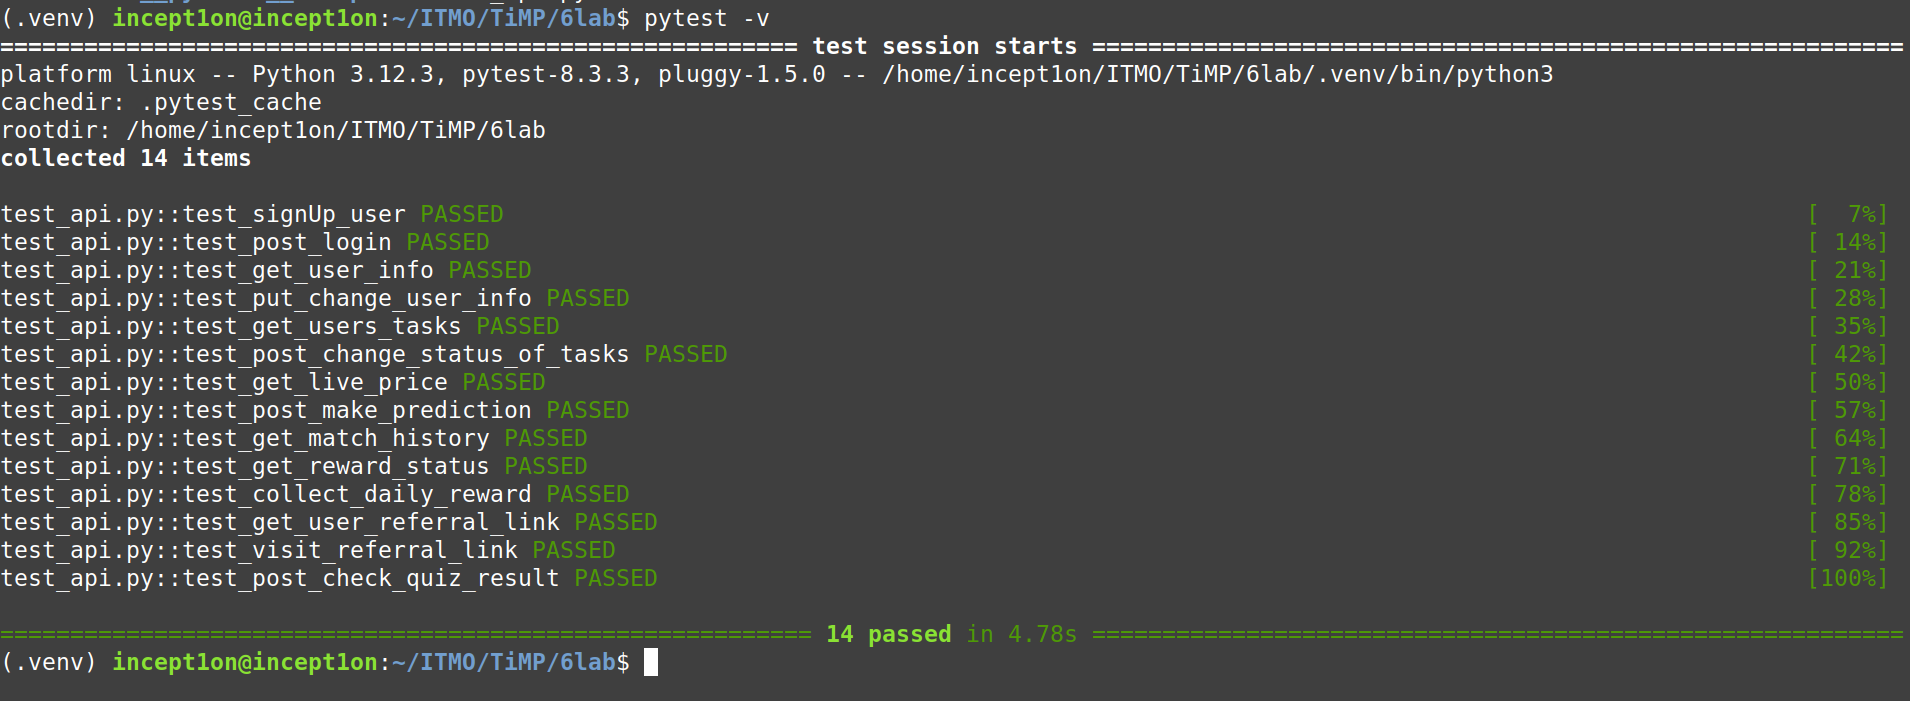
\includegraphics[width=1\linewidth]{pic_api_test.png}
    \caption{Удачное прохождение всех тестов}
    \label{fig:api_test}
\end{figure}

\subsection{Проверка на уязвимости}
Для проверки на уязвимости будет использоваться BurpSuitePro. Это приложение поможет перехватывать пакеты и изменять их на ходу.

В ходе исследования работы веб приложения cryptoroll.su, была выявлена одна неточность (баг) в его работе. По сценарию игры пользователь вводит сумму, которую он хочет поставить и дальше выбирает один из трёх вариантов времени, через которое он думает цена будет больше или меньше нынешней. Всего существует три варианта: 30 минут, 4 часа, 12 часов. Но программист, который разрабатывал приложение, для своего удобства, добавил скрытый для пользователя промежуток времени, который равняется 15 секундам. Следующие действия покажут как этого можно добиться.

Открываем сайт и BurpSuitePro и убеждаемся, что мы корректно видим все запросы.

\newpage
\begin{figure}[h!]
    \noindent
    \centering
    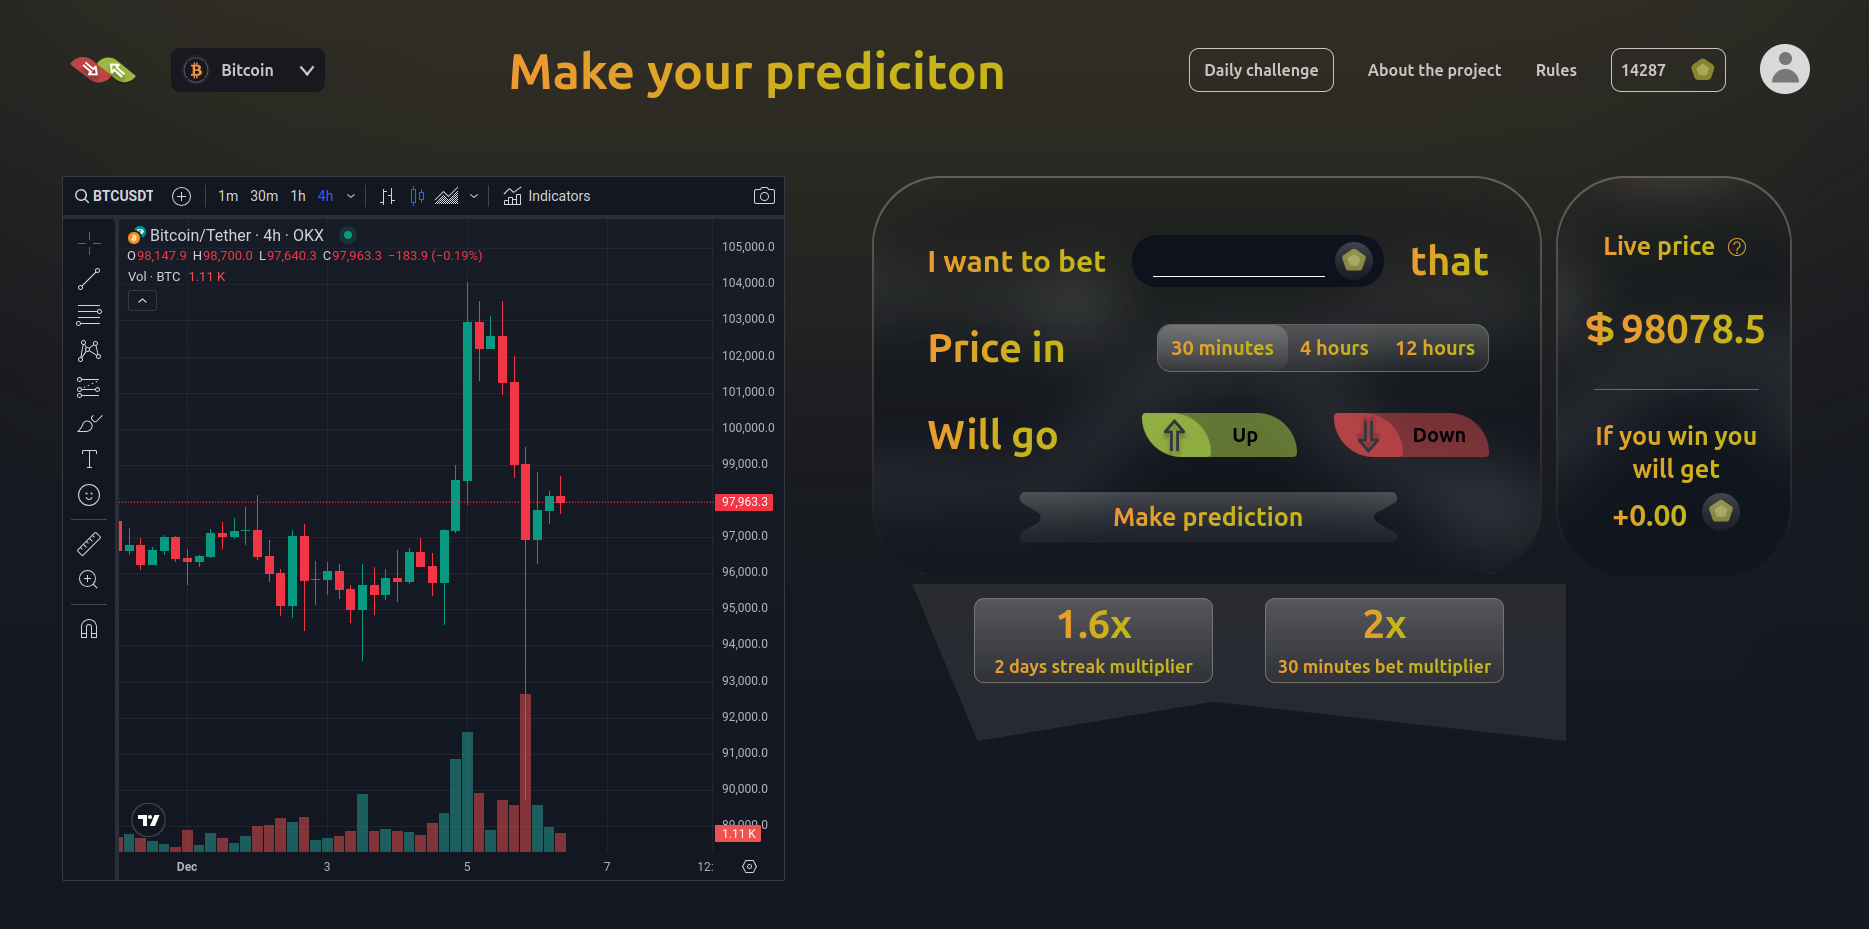
\includegraphics[width=1\linewidth]{pic_cryptoroll_1.png}
    \caption{Открываем cryptoroll.su}
\end{figure}

\begin{figure}[h!]
    \noindent
    \centering
    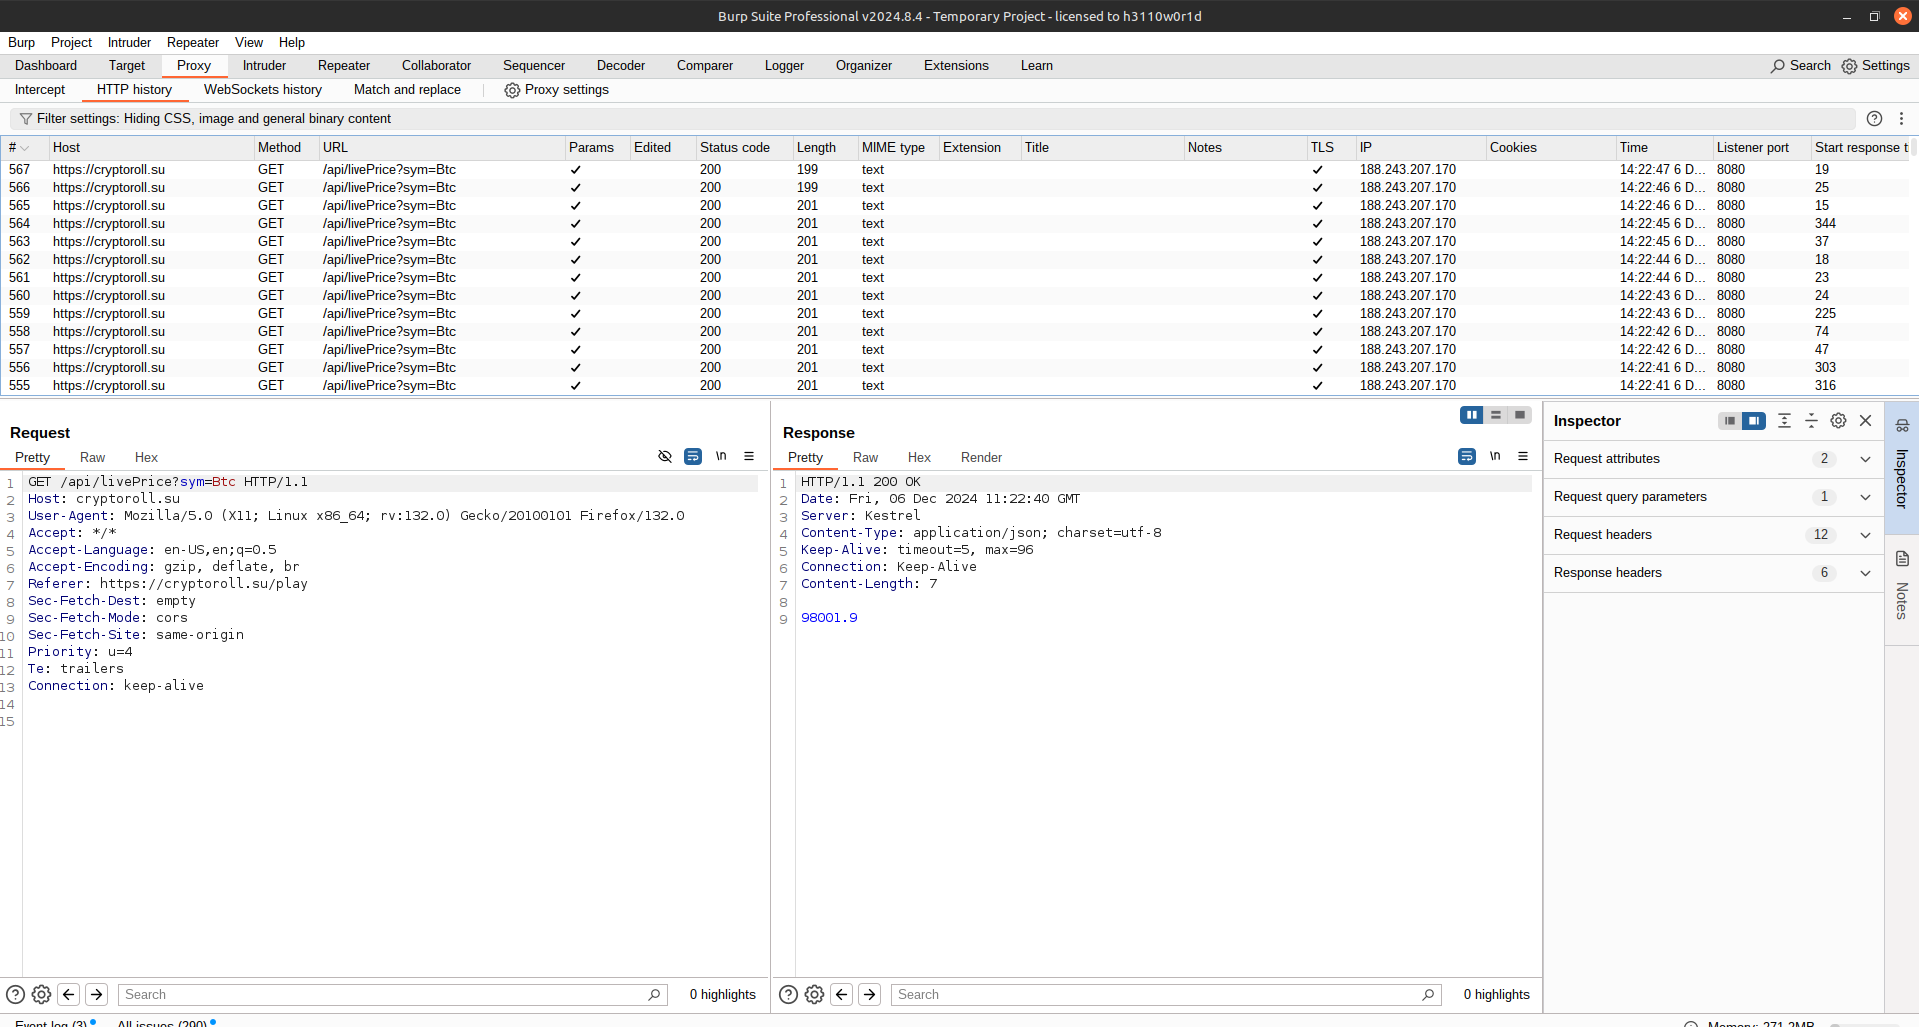
\includegraphics[width=1\linewidth]{pic_burp_1.png}
    \caption{Открываем BurpSuitePro}
\end{figure}

\newpage
\begin{figure}[h!]
    \noindent
    \centering
    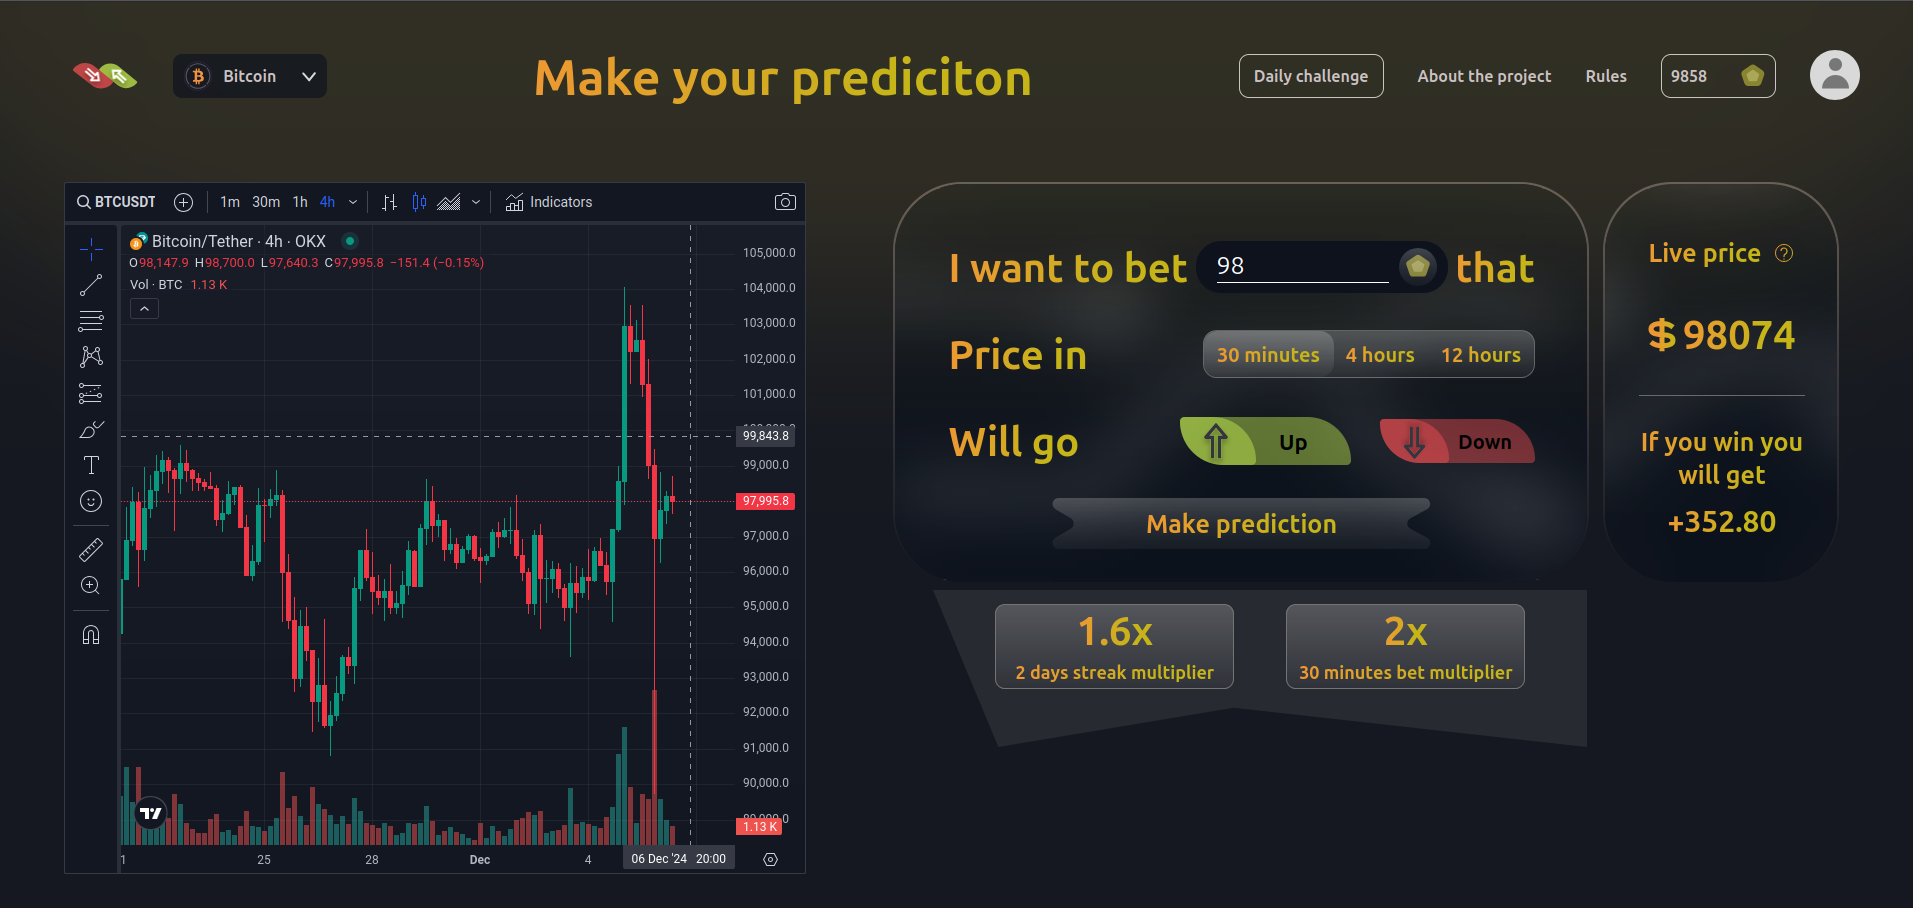
\includegraphics[width=1\linewidth]{pic_cryptoroll_2.png}
    \caption{Вводим произвольные данные}
\end{figure}

\begin{figure}[h!]
    \noindent
    \centering
    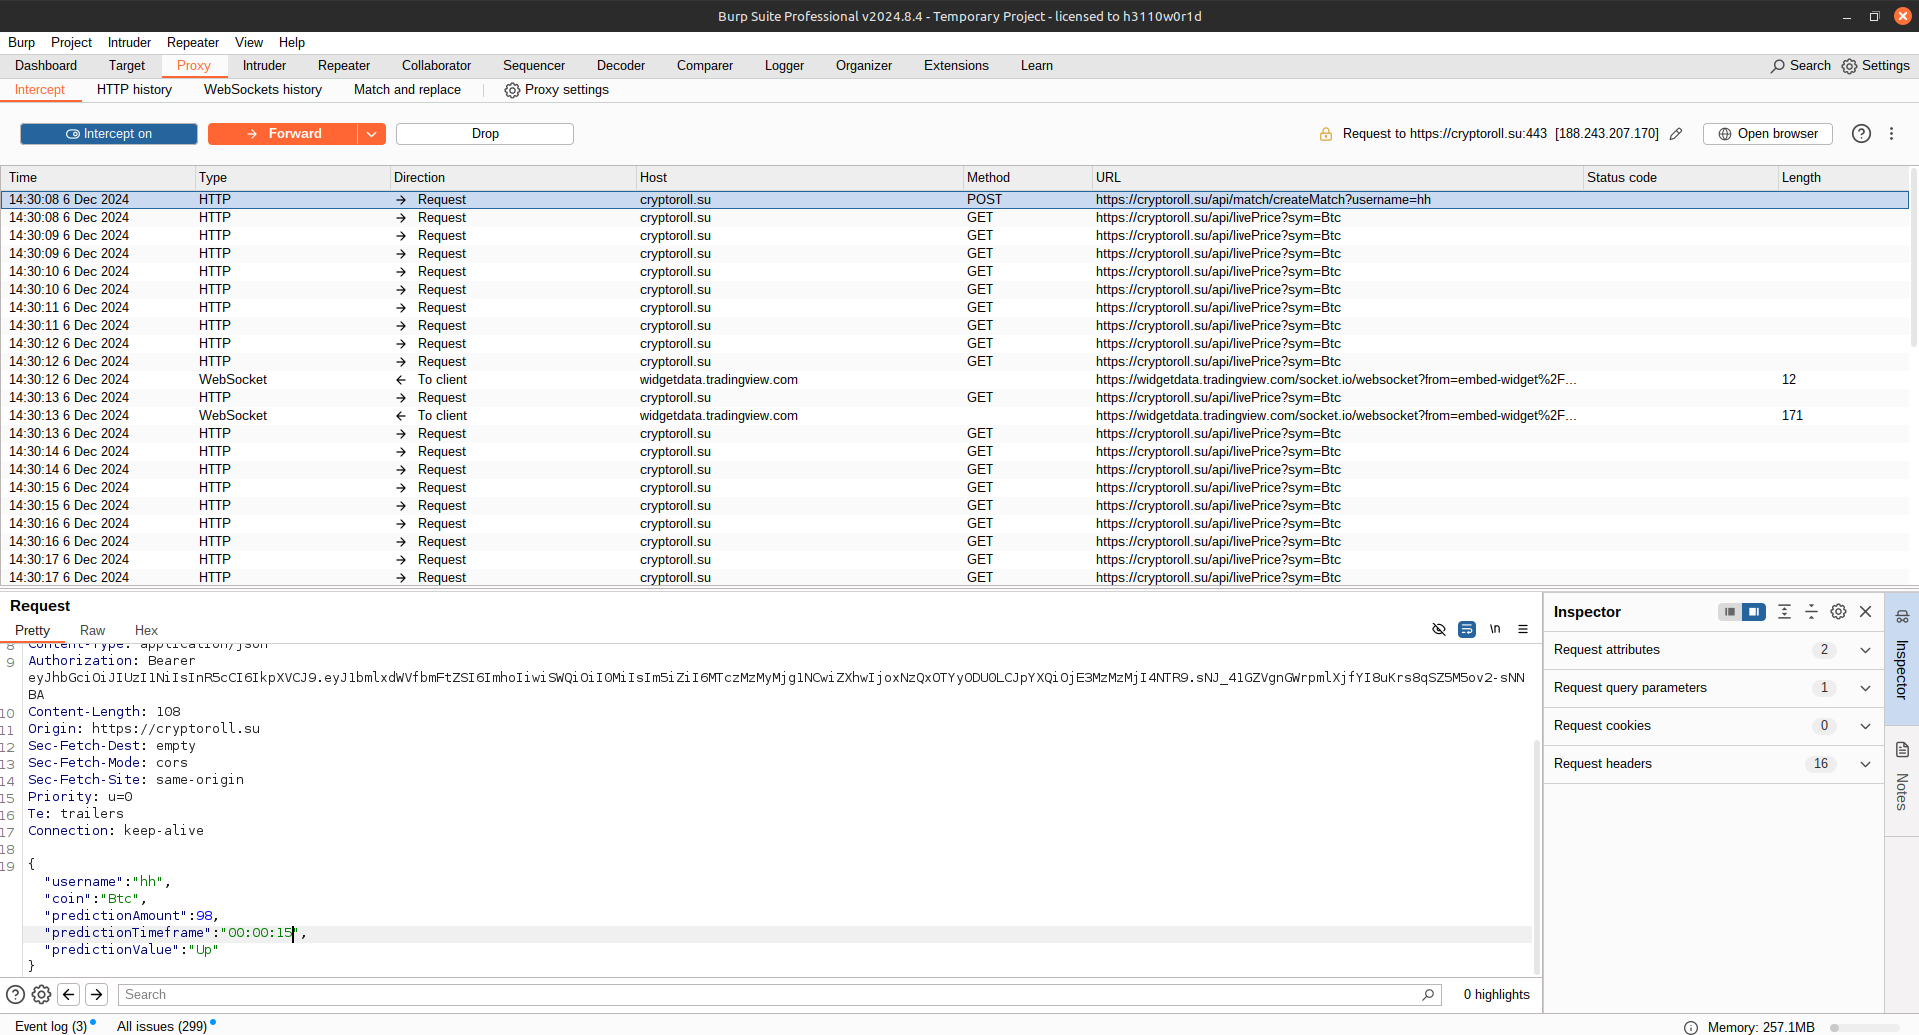
\includegraphics[width=1\linewidth]{pic_burp_2.png}
    \caption{Перехватываем POST запрос и меняем его тело}
\end{figure}

\newpage
\begin{figure}[h!]
    \noindent
    \centering
    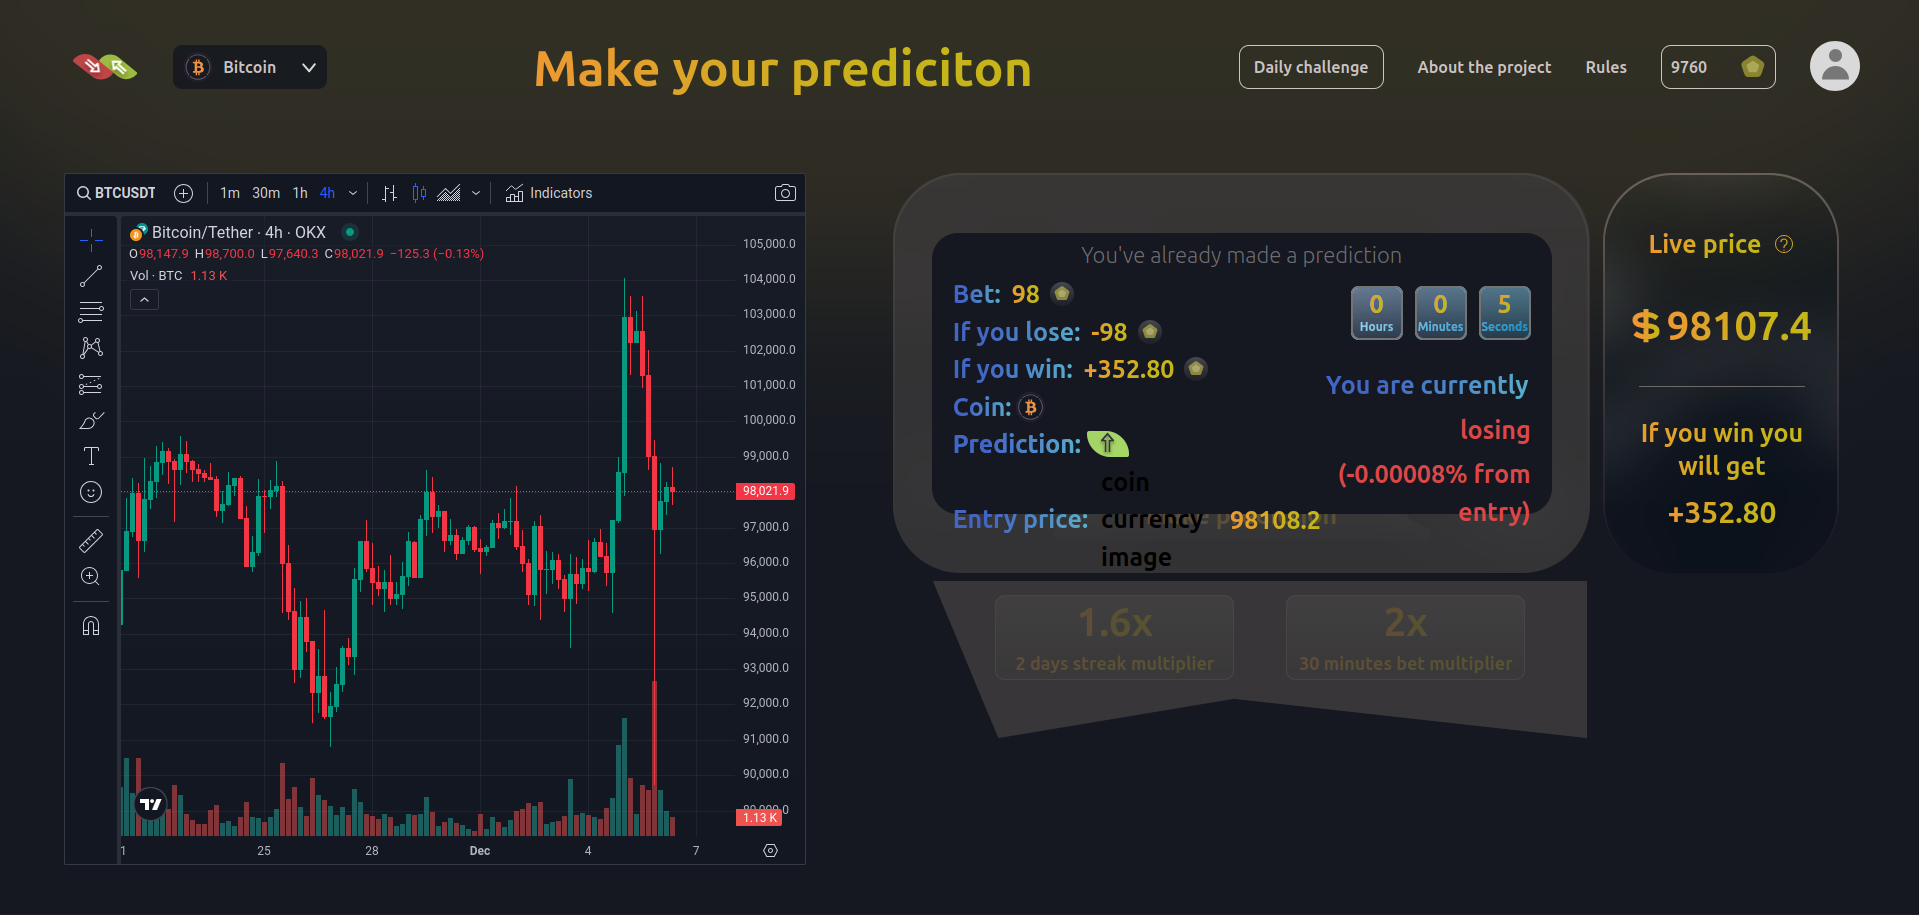
\includegraphics[width=1\linewidth]{pic_cryptoroll_3.png}
    \caption{Видим, что время, через которое должен выдаться результат меньше 15 секунд}
\end{figure}

\begin{figure}[h!]
    \noindent
    \centering
    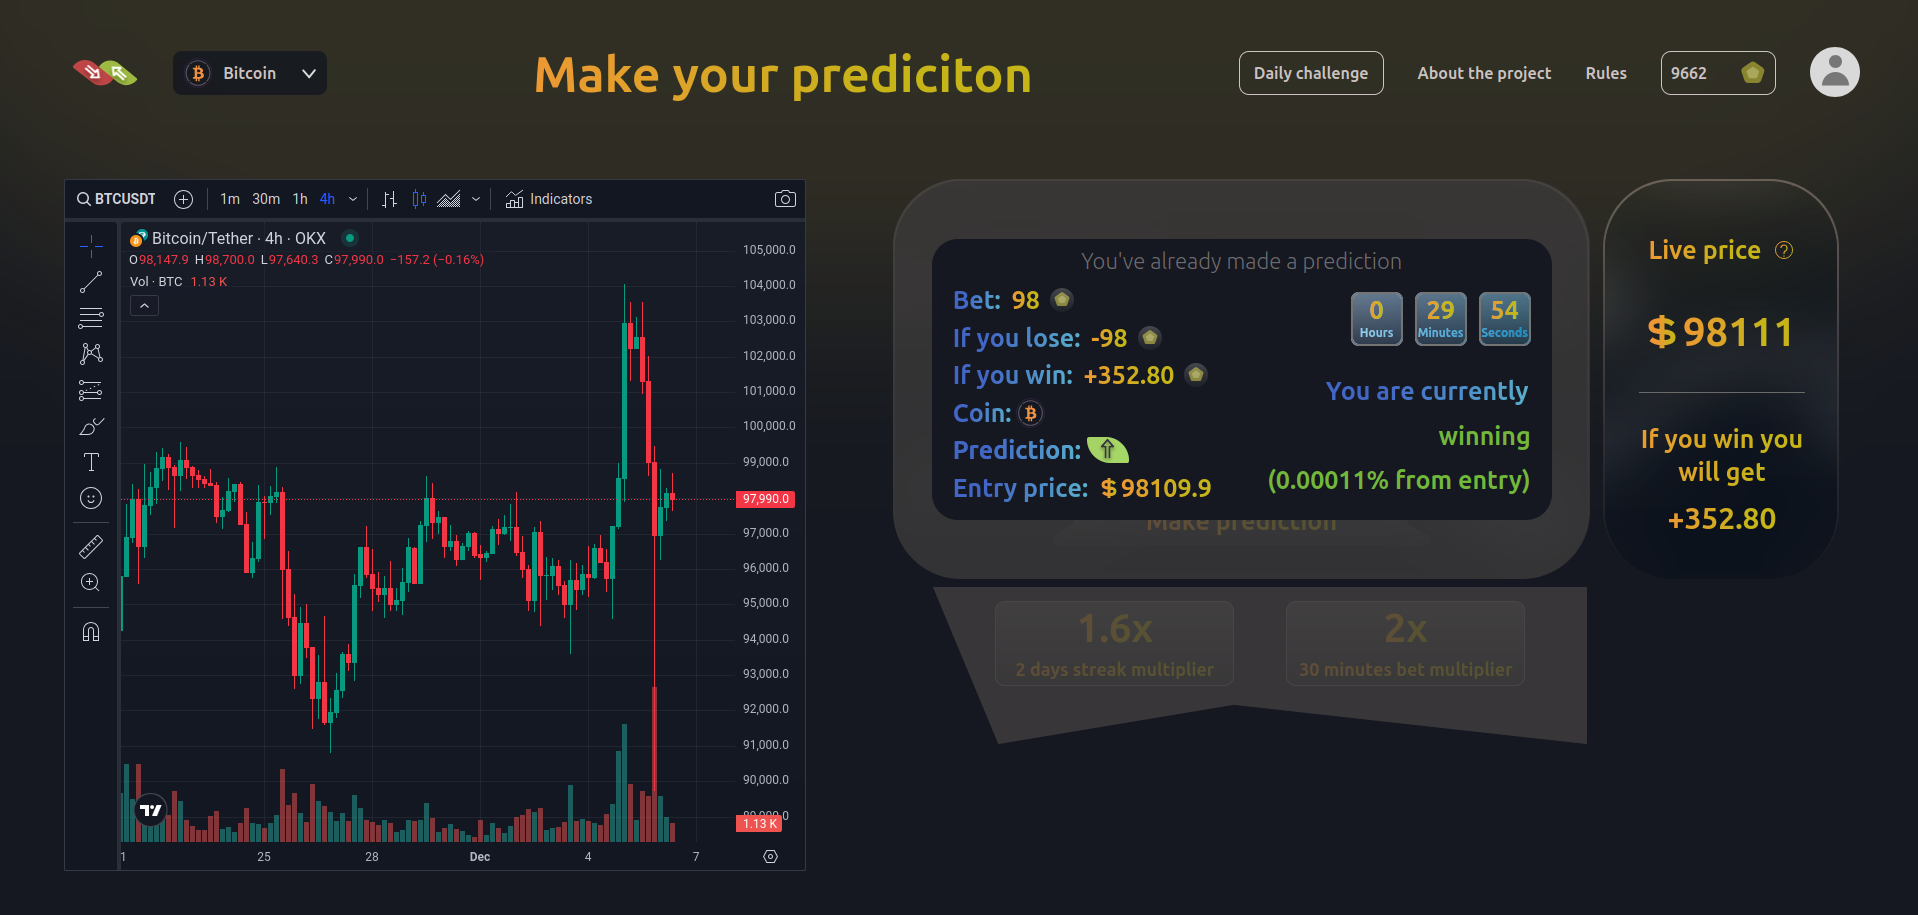
\includegraphics[width=1\linewidth]{pic_cryptoroll_4.png}
    \caption{Для сравнения пример нормально работающего приложения}
\end{figure}

\subsection{Проверка на нагрузку системы}

\textbf{Проверка нагрузки через троттлинг}

Через f12 в любом браузере, перейдя во вкладку Network, мы может в самом низу увидеть сколько времени нужно было, чтобы полностью загрузить сайт. (все дальнейшие тесты будут производиться нажимая сочетание клавиш ctr+f5, чтобы стирать весь кеш и имитировать первый заход пользователя)

\newpage
\begin{figure}[h!]
    \noindent
    \centering
    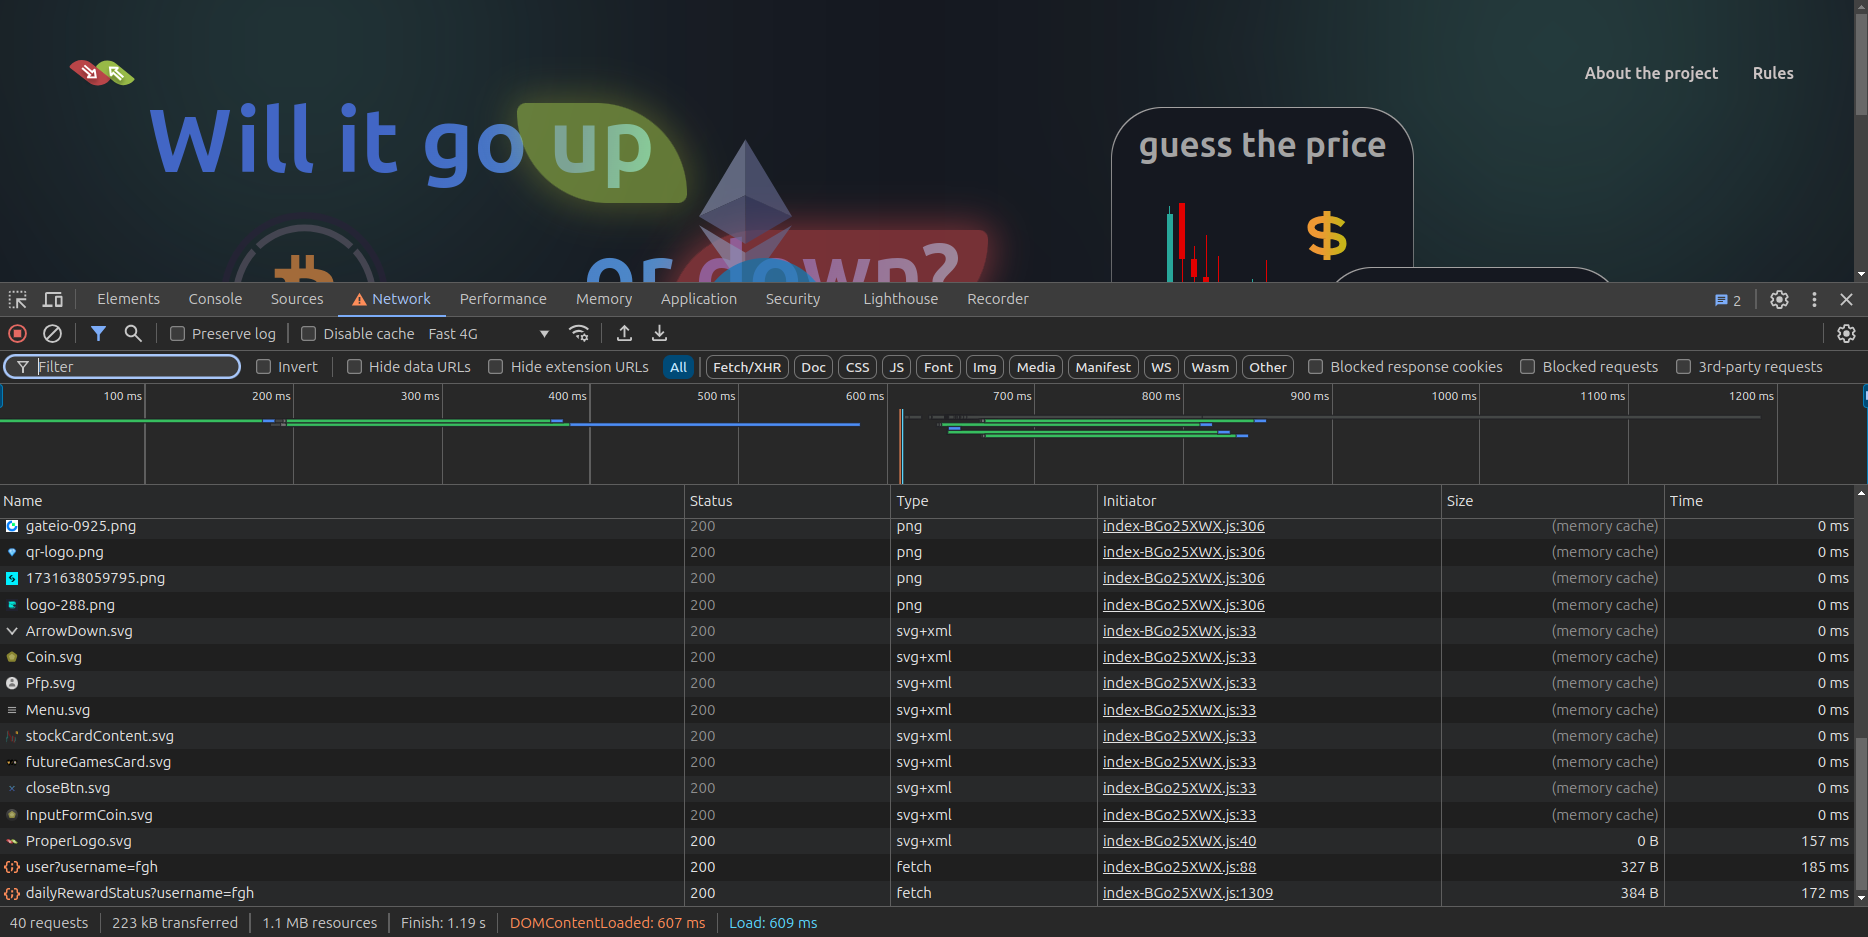
\includegraphics[width=1\linewidth]{pic_load_f12_1.png}
    \caption{load без троттлинга 609 мс}
\end{figure}

Выглядит всё очень даже хорошо, но теперь добавим троттлинг ''slow 4g и посмотрим на результат.

\begin{figure}[h!]
    \noindent
    \centering
    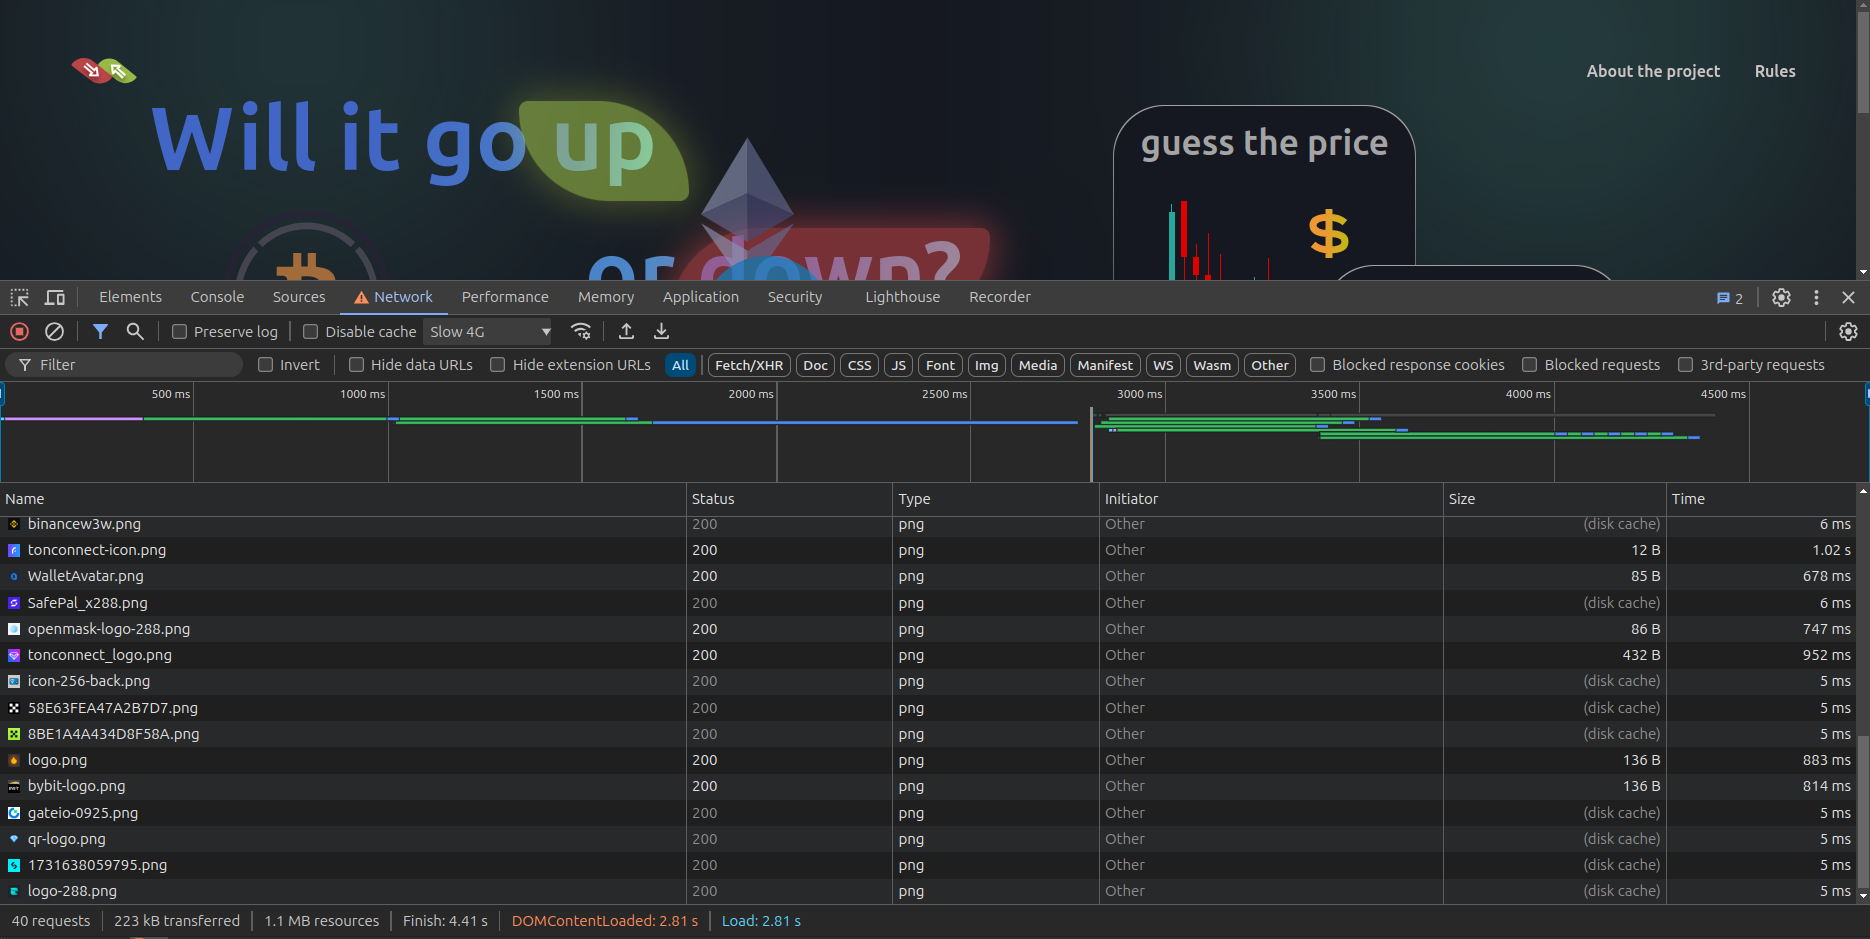
\includegraphics[width=1\linewidth]{pic_load_f12_2.png}
    \caption{load slow 4g 2.81 с}
\end{figure}

Видно, что даже небольшое замедление интернета у пользователя, и время загрузки увеличивается аж до 2.81 секунд (приличное время загрузки в бизнесе считается до трёх секунд).

Теперь увеличим троттлинг до 3g.

\newpage
\begin{figure}[h!]
    \noindent
    \centering
    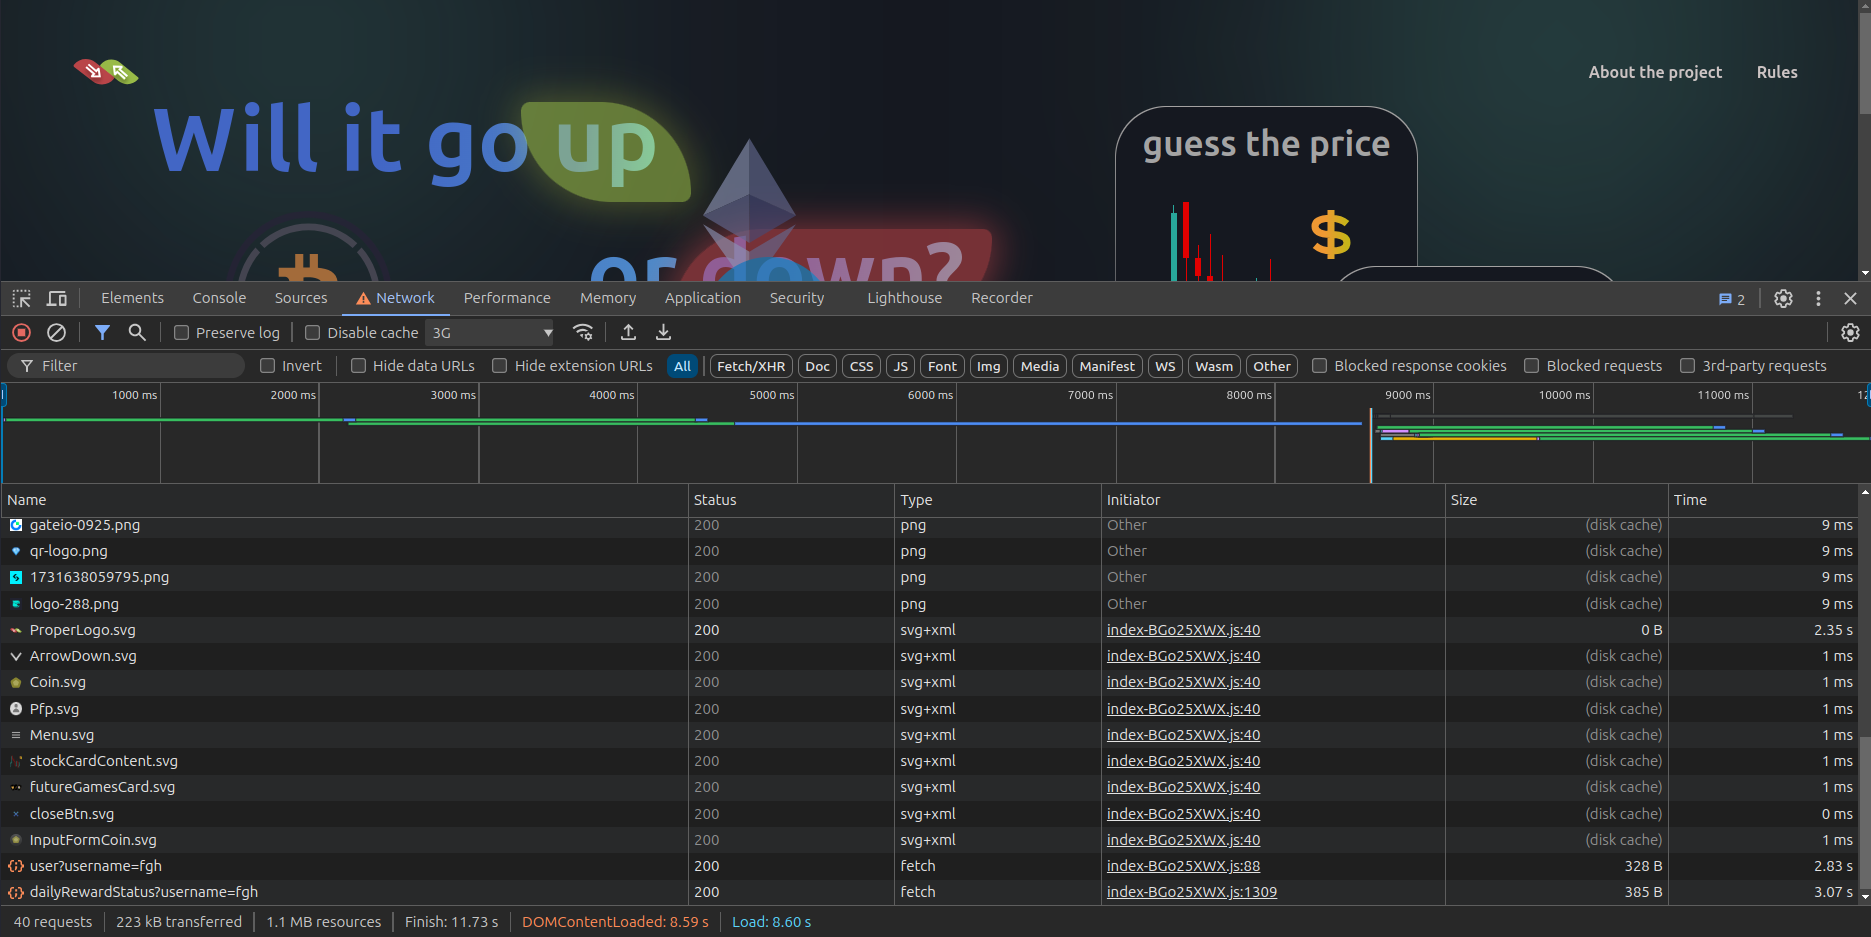
\includegraphics[width=1\linewidth]{pic_load_f12_3.png}
    \caption{load 3g 8.60 с}
\end{figure}

Видим, что теперь загрузка увеличилась до 8.60 секунд, что очень много, а это скорость без нагрузки в виде многих пользователей. Теперь выясним как мы можем сразу понять в чём проблема.

\textbf{Тестирование с помощью сайта для проверки нагрузки}

Воспользуемся сервисом \href{https://pagespeed.web.dev/?hl=ru}{pagespeed.web.dev}.

На сайте мы можем посмотреть различную статистику, включая первую загрузку какой-либо отрисовки, производительность на телефоне и компьютере и т.п. Но самое главное, что мы можем понять, что мы можем сделать для улучшения скорости загрузки сайта.

\begin{figure}[h!]
    \noindent
    \centering
    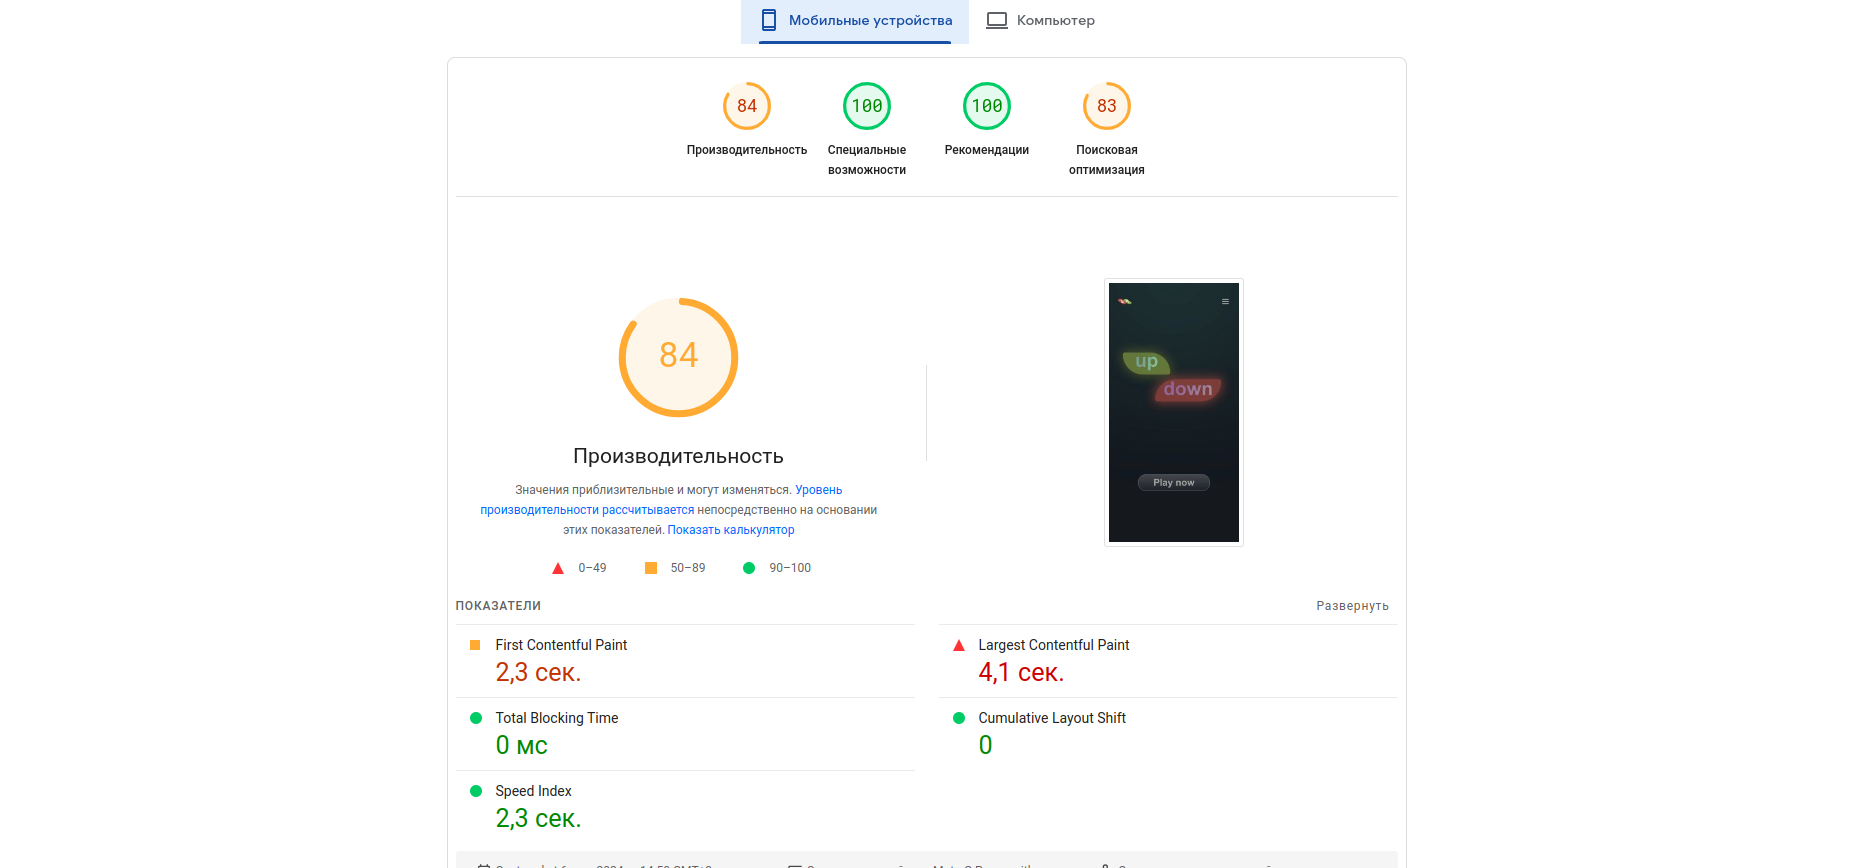
\includegraphics[width=1\linewidth]{pic_web_1.png}
    \caption{Производительность на телефоне}
\end{figure}

\newpage
\begin{figure}[h!]
    \noindent
    \centering
    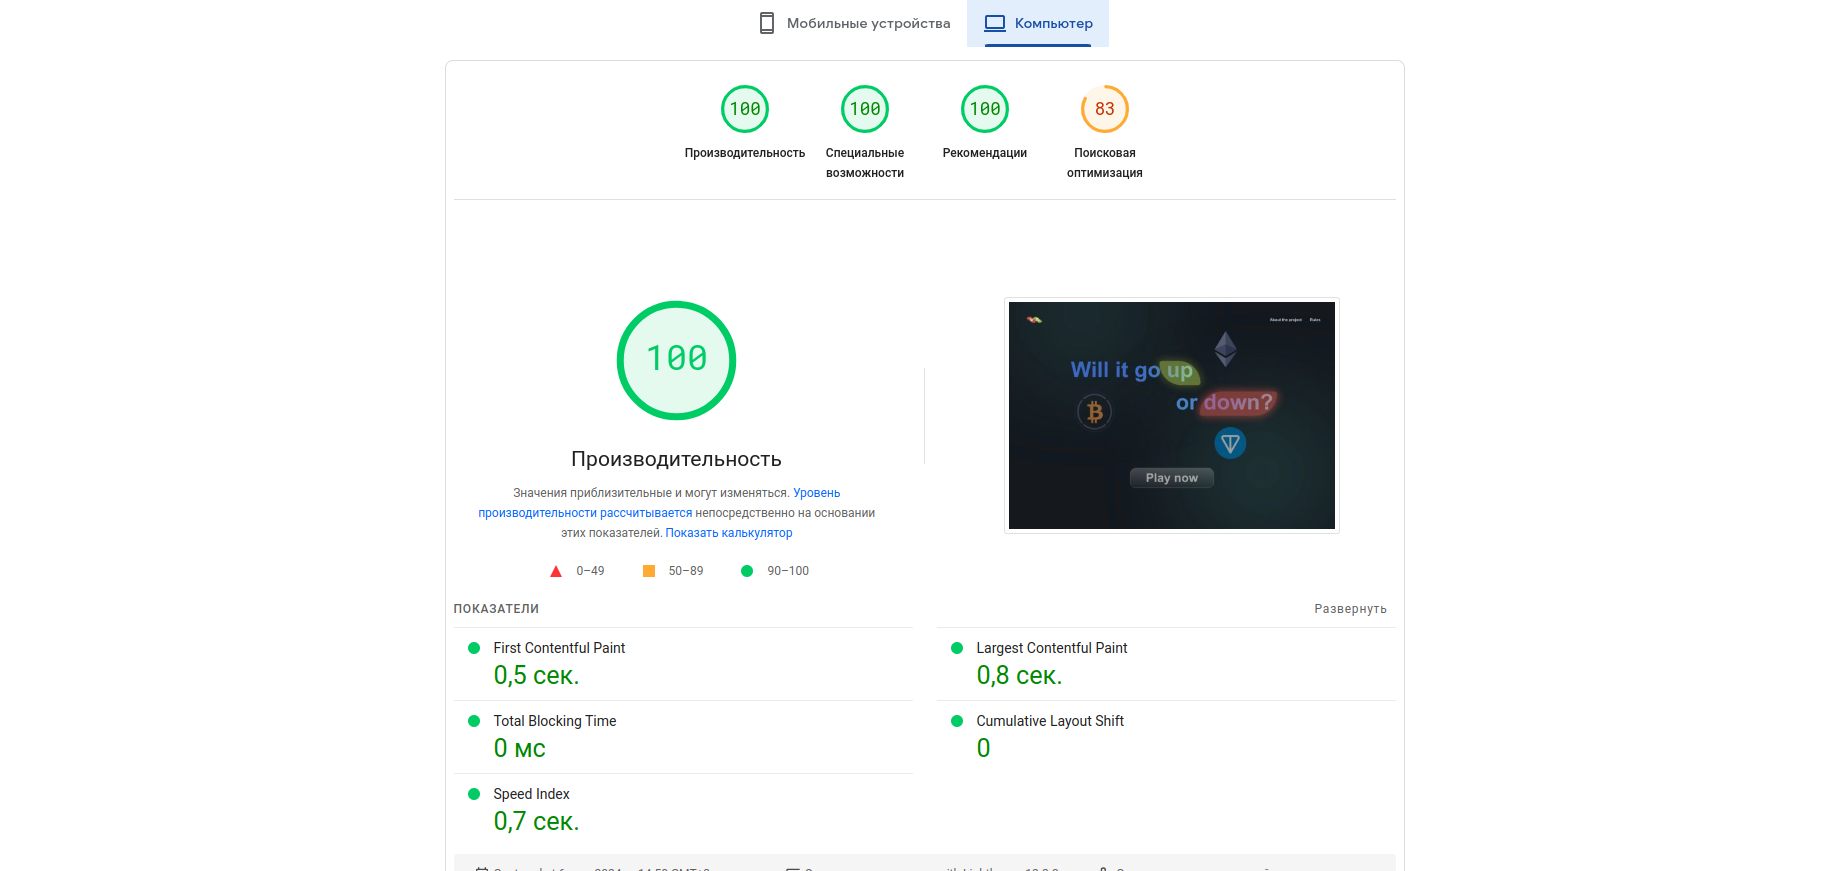
\includegraphics[width=1\linewidth]{pic_web_2.png}
    \caption{Производительность на компьютере}
\end{figure}

\begin{figure}[h!]
    \noindent
    \centering
    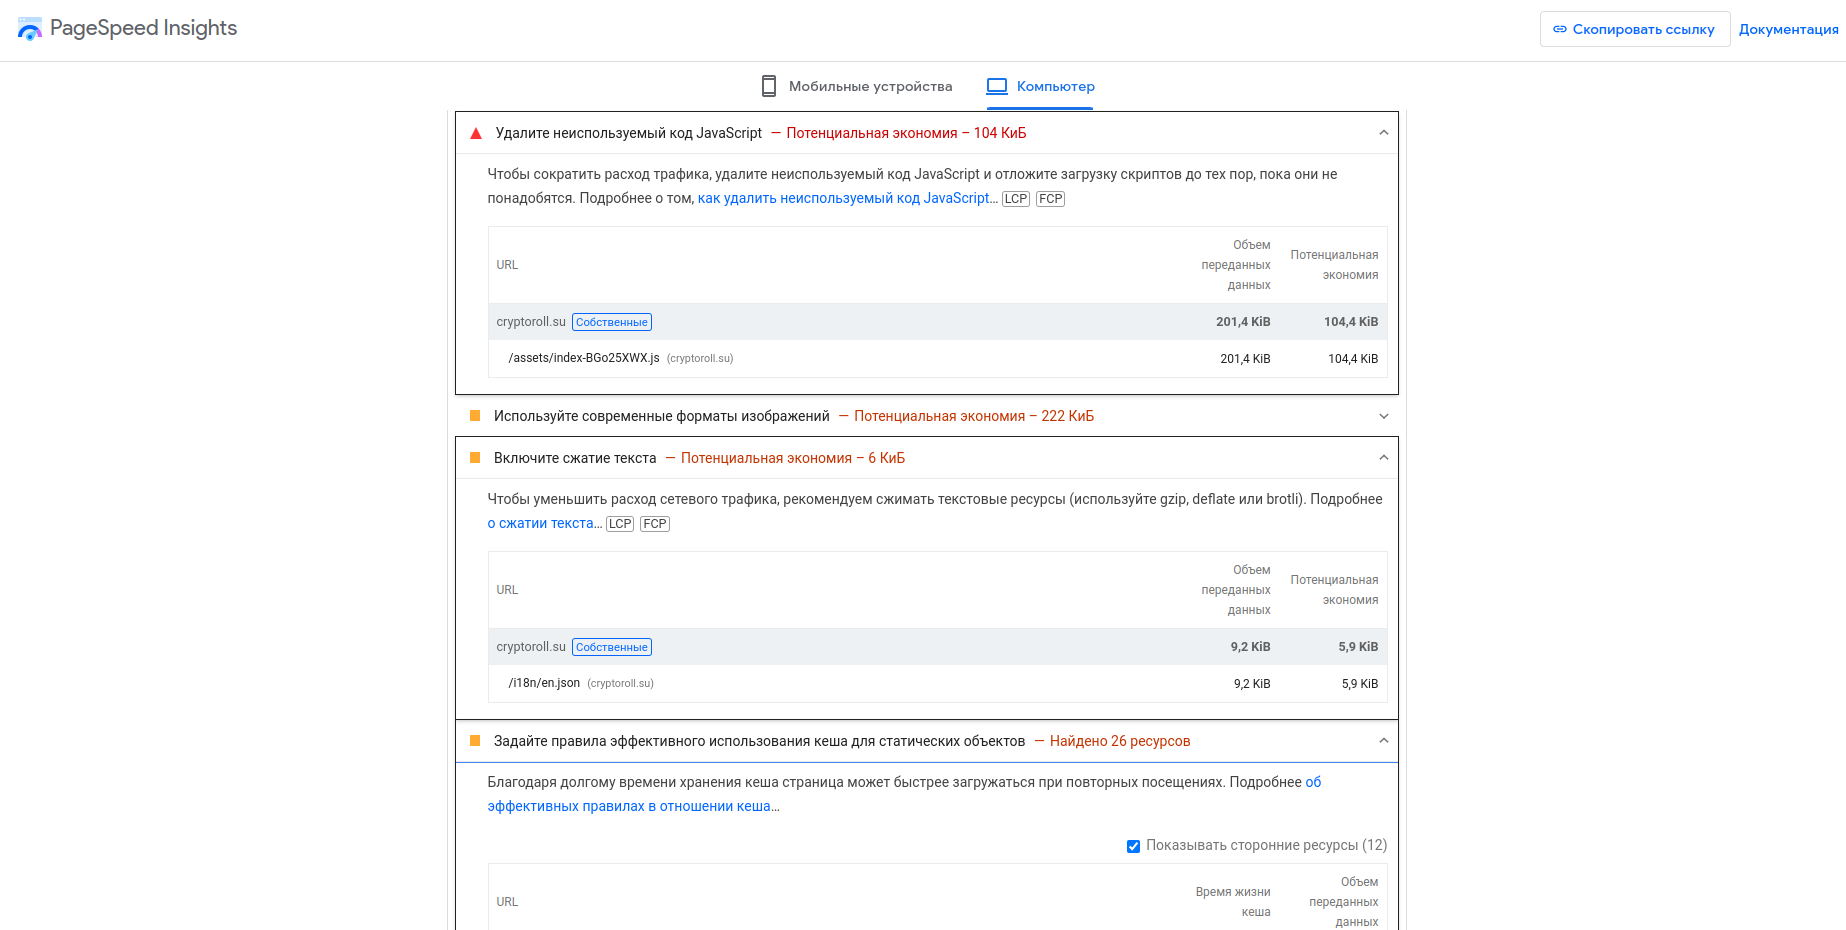
\includegraphics[width=1\linewidth]{pic_web_3.png}
    \caption{Некоторые советы по улучшению скорости загрузки}
\end{figure}

\textbf{Тестирование нагрузки для нескольких пользователей}

Теперь протестируем работу приложения под нагрузкой. Воспользуемся встроенной Linux утилитой Apache benchmark. Она позволяет отправлять несколько запросов на ресурс многопоточно, что позволяет оценить насколько хорошо сервер справляется с нагрузкой.

Протеститруем лендинговую страницу cryptoroll.su, подав на вход в утилиту 600 запросов с многопоточностью в 200 запросов.

\newpage
\begin{figure}[h!]
    \noindent
    \centering
    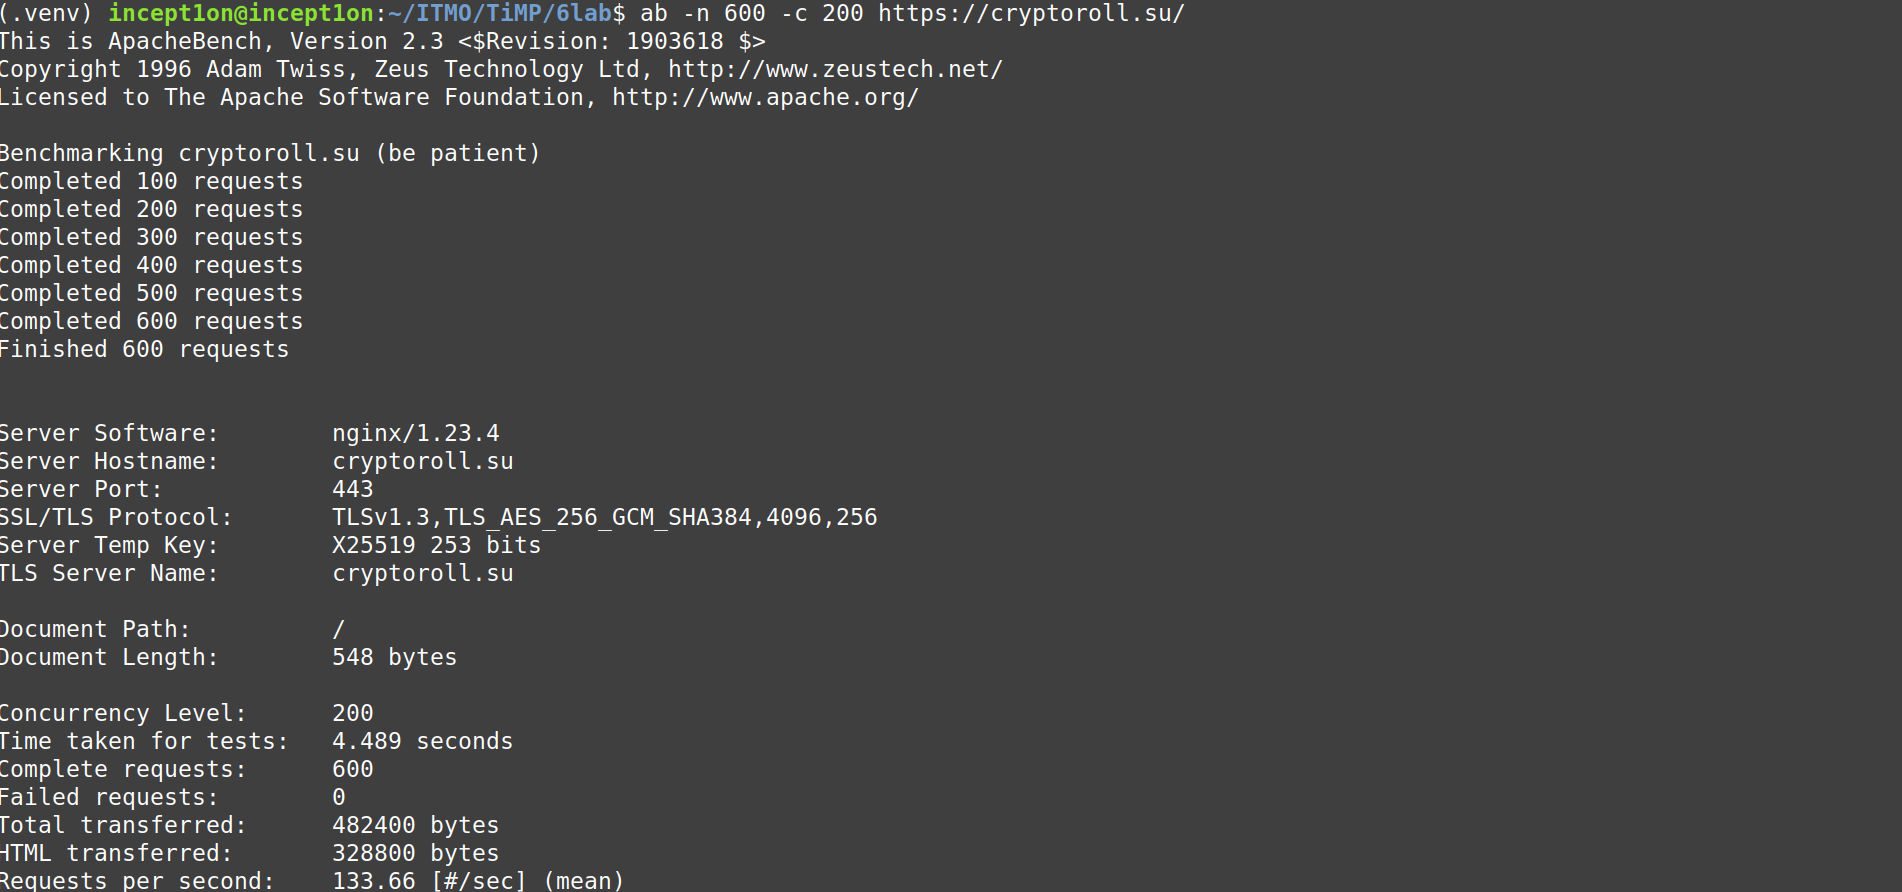
\includegraphics[width=1\linewidth]{pic_ab_1.png}
    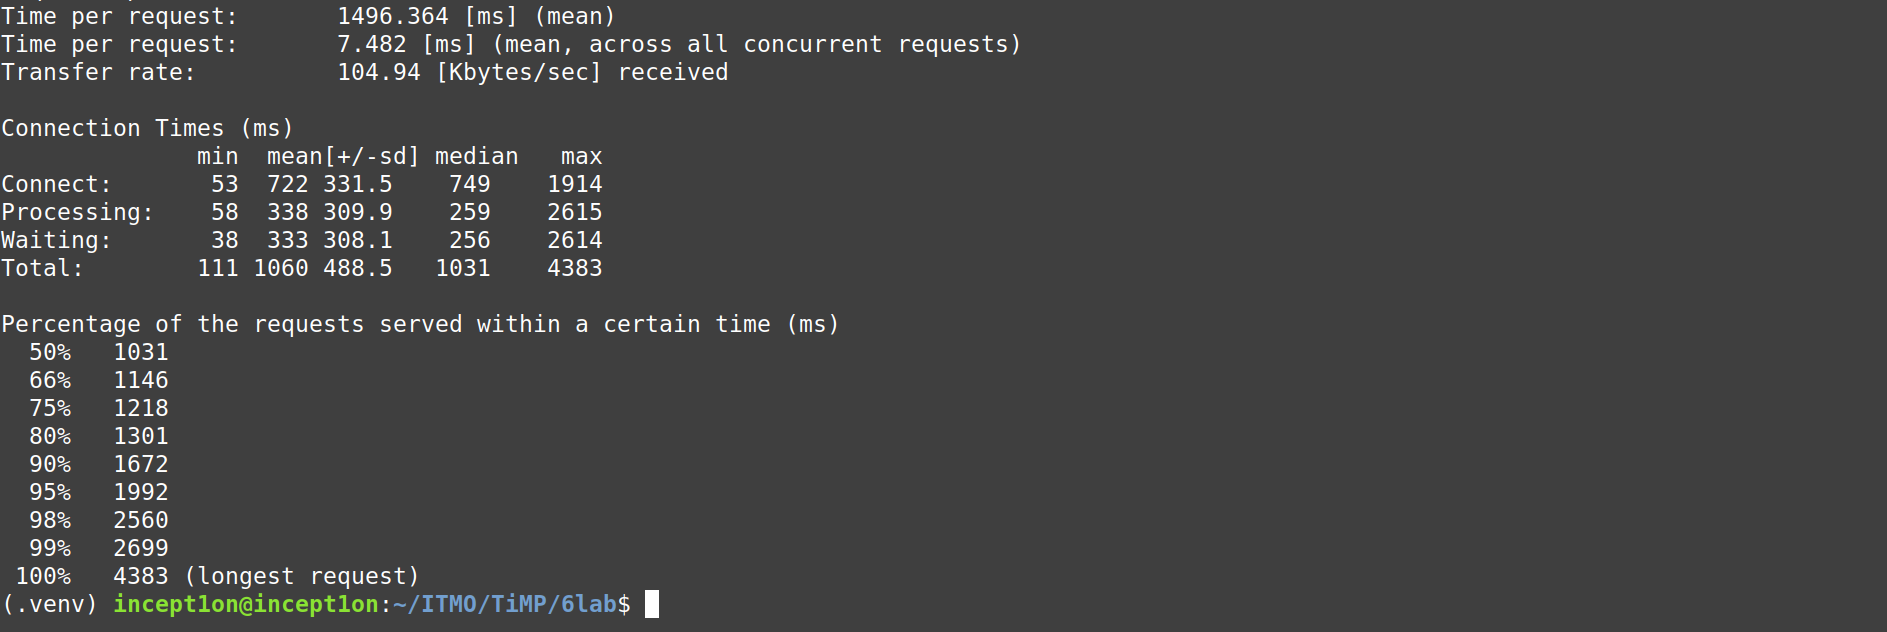
\includegraphics[width=1\linewidth]{pic_ab_2.png}
    \caption{Работа утилиты Apache Benchmark}
\end{figure}

Здесь есть несколько ключевых моментов, на которые надо обратить внимание:
\begin{enumerate}
    \item Failed requests - количество запросов, которые не были обработаны.
    \item Time per request (mean) - среднее количество, которое потребовалось на загрузку страницы.
    \item Total (max) - максимальное время, которое потребовалось для загрузки страницы.
\end{enumerate}

В примере выше все запросы были удачно обработаны, среднее время на загрузку страницы было примерно 1.5 секунды и максимальное время загрузки примерно 4 секунды. Все параметры выглядят в норме, кроме максимального времени загрузки, 4 секунды означает, что мы можем потерять некоторых пользователей, которые зашли на страницу.

Попробуем ещё сильнее увеличить нагрузку, подав на вход 3000 запросов с многопоточность в 600 запросов.

\newpage
\begin{figure}[h!]
    \noindent
    \centering
    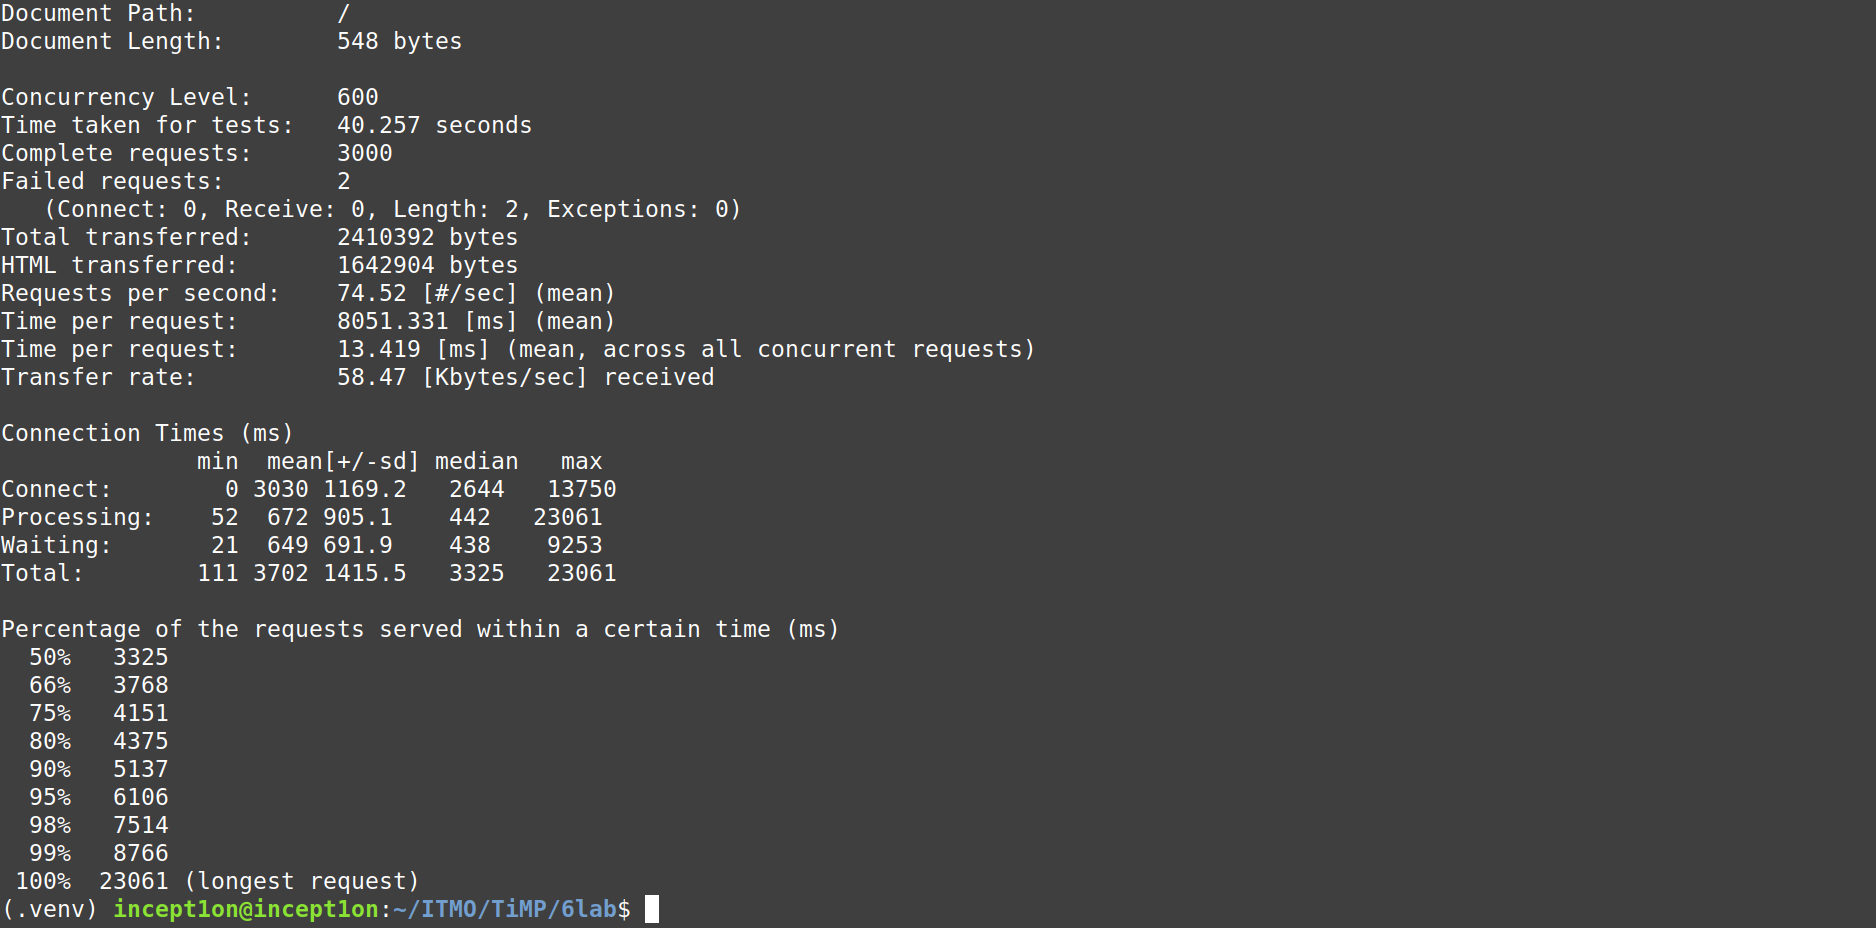
\includegraphics[width=1\linewidth]{pic_ab_3.png}
    \caption{Результат после увеличения нагрузки}
\end{figure}

Мы видим, что из 3000 запросов 2 запроса были ''Failed'', среднее время ожидания на загрузку было 8, а максимальное 23 секунды. Это уже выглядит как очень плохой результат.

При дальнейшей нагрузке количество неудачных запросов будет увеличиваться до тех пор, пока сервис не перестанет быть доступным.

''Failed requests'' означает, что процессор не справляется с нагрузкой, это означает, что чтобы решить данную проблему надо выделить больше ядер для данной виртуальной машины.

\textbf{Проверка доступности сервера из разных уголков мира}

Есть сервисы, которые позволяют проверить сколько времени понадобиться людям в различных странах, чтобы загрузить файлы сайта. Воспользуемся сревисом \href{https://check-host.net/check-http?lang=ru}{check-host.net/check-http}

\newpage
\begin{figure}[h!]
    \noindent
    \centering
    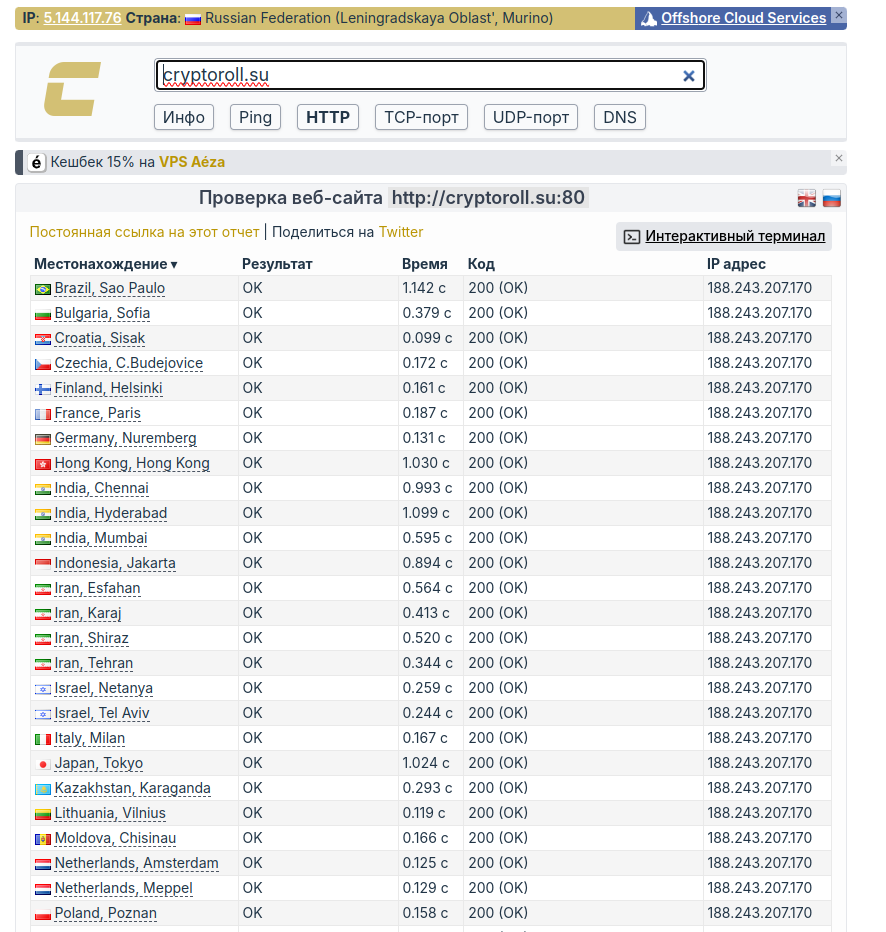
\includegraphics[width=1\linewidth]{pic_ping_1.png}
    \caption{}
\end{figure}

\newpage
\begin{figure}[h!]
    \noindent
    \centering
    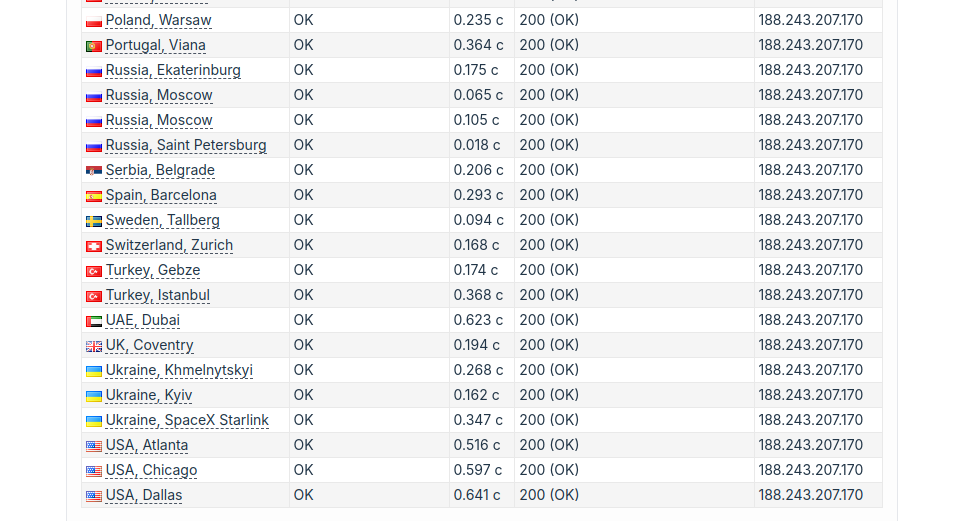
\includegraphics[width=1\linewidth]{pic_ping_2.png}
    \caption{}
\end{figure}

Можно увидеть, что сайт хорошо доступен по всему миру. Самое долгое время загрузки потребовалось для Индии, Гонконга и Бразилии, время ответа для этих районов составило чуть больше 1 секунды.

\newpage
\section{Заключение}

В результате лабораторной работы было проведено тестирование сервиса\\ cryptoroll.su. Были получены теоретические и практические навыки способов тестирования. 

Было произведено тестирования API, тестирование на уязвимость и тестирование нагрузки в различных формах. Было описано как решить и исправить выявленные недостатки.




\newpage
\section{Приложение}
\begin{lstlisting}[language=python, caption={Код для тестирования API}]
import string
import requests
import random

def randomString(length=10):
    characters = string.ascii_letters + string.digits
    return ''.join(random.choice(characters) for _ in range(length))

baseUrl = "https://cryptoroll.su/api"
jwt_token = None
login = randomString()
passwd = randomString()


def test_signUp_user():
    global login
    global passwd

    body = {
        "username":f"{login}",
        "password":f"{passwd}"
    }

    response = requests.post(url=f"{baseUrl}/signup", json=body)
    assert response.status_code == 201, f"Error! Status code = {response.status_code}"

    dataOfResponse = response.json()
    jwt_token = dataOfResponse.get('jwtToken')
    assert jwt_token, "Error! JWT token was not provided"
    
    

def test_post_login():
    global jwt_token
    global login
    global passwd

    data={
    "username": f"{login}",
    "password": f"{passwd}"
    }

    response = requests.post(f"{baseUrl}/login", json=data)
    assert response.status_code == 201, f"Error! Response code is {response.status_code}"
    dataResponse = response.json()
    user = dataResponse.get('user', {})
    jwt_token = dataResponse.get('jwtToken')

    assert user, "User is empty"
    assert jwt_token, "User is empty"

    name = user.get('name')
    assert name == login

def test_get_user_info():
    global jwt_token
    global login

    token = jwt_token

    headers = {
        'Authorization': f'Bearer {token}',
    }

    response = requests.get(f"{baseUrl}/user?username={login}", headers=headers)
    dataOfResponse = response.json()

    assert response.status_code == 200, f"Error! Status code is {response.status_code}"
    assert dataOfResponse, "Error! The recieved data is empty"

    username = dataOfResponse.get('username')
    assert username == login

def test_put_change_user_info():
    global jwt_token
    global login

    data = {
    "name": "haha",
    "password": f"{passwd}",
    "walletAddress": "hehe"
    }

    token = jwt_token

    headers = {
        'Authorization': f'Bearer {token}',
    }

    response = requests.put(f"{baseUrl}/user?username={login}", json=data, headers=headers)
    assert response.status_code == 200, f"Error! Status code: {response.status_code}"
    dataOfResponse = response.json()

    newToken = dataOfResponse.get("newToken")
    assert newToken != token
    jwt_token = newToken

    data = {
    "name": f"{login}",
    "password": f"{passwd}",
    "walletAddress": "hehe"
    }

    token = jwt_token

    headers = {
        'Authorization': f'Bearer {token}',
    }

    response = requests.put(f"{baseUrl}/user?username=haha", json=data, headers=headers) 
    assert response.status_code == 200, f"Status code: {response.status_code}"
    dataOfResponse = response.json()

    newToken = dataOfResponse.get("newToken")
    assert newToken != token
    jwt_token = newToken


def test_get_users_tasks():
    global jwt_token
    global login

    token = jwt_token

    headers = {
        'Authorization': f'Bearer {token}',
    }    

    response = requests.get(url=f"{baseUrl}/tasks?username={login}", headers=headers)
    assert response.status_code == 200, f"Error! Status code is {response.status_code}"

    dataOfResponse = response.json()
    assert dataOfResponse, "No data recieved"



def test_post_change_status_of_tasks():
    global jwt_token
    global login

    token = jwt_token

    headers = {
        'Authorization': f'Bearer {token}',
    }    
    response = requests.get(url=f"{baseUrl}/tasks?username={login}", headers=headers)
    assert response.status_code == 200, f"Error! Status code is {response.status_code}"
    dataOfResponse = response.json()
    tasksInfo = dataOfResponse.get('tasks', [])
    statusTastOne = tasksInfo[0].get('status')
    assert statusTastOne == "Uncompleted"

    body = {
    "taskId": 1,
    "changedStatus": "Completed"
    }

    headers = {
        'Authorization': f'Bearer {token}',
    }    

    response = requests.post(url=f"{baseUrl}/tasks?username={login}", json= body, headers=headers)
    assert response.status_code == 200, f"Error! Status code is {response.status_code}"

    response = requests.get(url=f"{baseUrl}/tasks?username={login}", headers=headers)
    assert response.status_code == 200, f"Error! Status code is {response.status_code}"
    dataOfResponse = response.json()
    tasksInfo = dataOfResponse.get('tasks', [])
    statusTastOne = tasksInfo[0].get('status')
    assert statusTastOne == "Completed"

    
def test_get_live_price():
    global login

    response = requests.get(f"{baseUrl}/livePrice?sym=Btc")
    assert response.status_code == 200, f"Error! Status code is {response.status_code}"

    dataOfResponse = response.text
    assert dataOfResponse, f"Error! The price is {dataOfResponse}"

def test_post_make_prediction():
    global jwt_token
    global login

    token = jwt_token

    body = {
        "username": f"{login}",
        "coin": "Btc",
        "predictionAmount": 10,
        "predictionTimeframe": "00:30:00",
        "predictionValue": "Up"
    }

    headers = {
        'Authorization': f'Bearer {token}',
    }    

    response = requests.post(url=f"{baseUrl}/match/createMatch?username={login}", json=body, headers=headers)

    assert response.status_code == 204, f"Error! Status code is {response.status_code}"

    response = requests.post(url=f"{baseUrl}/match/createMatch?username={login}", json=body, headers=headers)

    assert response.status_code == 400, f"Error! Status code is {response.status_code}"

def test_get_match_history():
    global jwt_token
    global login

    token = jwt_token

    headers = {
        'Authorization': f'Bearer {token}',
    }    

    response = requests.get(url=f"{baseUrl}/match/history?username={login}&offset=0&limit=10", headers=headers)
    assert response.status_code == 200, f"Error! Status code is {response.status_code}"

def test_get_reward_status():
    global jwt_token
    global login

    token = jwt_token

    headers = {
        'Authorization': f'Bearer {token}',
    }    

    response = requests.get(url=f"{baseUrl}/rewards/dailyRewardStatus?username={login}", headers=headers)
    assert response.status_code == 200, f"Error! Status code is {response.status_code}"
    assert response.json()

def test_collect_daily_reward():
    global jwt_token
    global login

    token = jwt_token

    headers = {
        'Authorization': f'Bearer {token}',
    }    

    response = requests.get(url=f"{baseUrl}/rewards/dailyRewardStatus?username={login}", headers=headers)
    assert response.status_code == 200, f"Error! Status code is {response.status_code}"
    assert response.text

def test_get_user_referral_link():
    global jwt_token
    global login

    token = jwt_token

    headers = {
        'Authorization': f'Bearer {token}',
    }    

    response = requests.get(url=f"{baseUrl}/referralLinks/?username={login}", headers=headers)
    assert response.status_code == 200, f"Error! Status code is {response.status_code}"
    assert response.__str__, f"Error! The response is {response}"

def test_visit_referral_link():
    global jwt_token
    global login

    token = jwt_token

    headers = {
        'Authorization': f'Bearer {token}',
    }    

    salt = requests.get(url=f"{baseUrl}/referralLinks/?username={login}", headers=headers).__str__
    
    response = requests.post(url=f"{baseUrl}/referralLinks/visit?visitorName=hehe&referralSalt={salt}", headers=headers)

    assert response.status_code == 403, f"Error! The status code is {response.status_code}"

def test_post_check_quiz_result():
    global jwt_token
    global login

    token = jwt_token

    headers = {
        'Authorization': f'Bearer {token}',
    }    

    body = [
    {
        "questionId": 1,
        "questionAnswer": 0
    },
    {
        "questionId": 2,
        "questionAnswer": 3
    },
    {
        "questionId": 3,
        "questionAnswer": 2
    },
    {
        "questionId": 4,
        "questionAnswer": 2
    },
    {
        "questionId": 5,
        "questionAnswer": 1
    }
    ]

    [
    {
        "questionId": 1,
        "questionAnswer": 0
    },
    {
        "questionId": 2,
        "questionAnswer": 3
    },
    {
        "questionId": 3,
        "questionAnswer": 2
    },
    {
        "questionId": 4,
        "questionAnswer": 2
    },
    {
        "questionId": 5,
        "questionAnswer": 1
    }
]

    response = requests.post(url=f"{baseUrl}/quiz?username={login}", headers=headers, json=body)
    assert response.status_code == 200, f"Error! The status code is {response.status_code}"

    dataOfResponse = response.json()
    isQuizCompleted = dataOfResponse.get('isQuizCompleted')
    assert isQuizCompleted == False    
    
\end{lstlisting}


\end{document}